\section{Welfare and the deadweight loss of market power}\label{sec:02-welfare}

The previous sections asked how far price exceeds marginal cost and why. This section asks what the gap costs
society. A positive correlation between concentration and margins, or an estimated conduct parameter above zero,
does not by itself tell us that the losses are large. To answer the normative question we need a measure of welfare,
a way to compute it from demand and cost, and a sense of its likely size. We first set up the standard
partial-equilibrium apparatus and derive closed forms for linear demand. We then present the Harberger
approximation and the debate it started. The section closes with three qualifications: production inefficiency
across firms, entry, and the trade-off between market power and cost savings in mergers.

\subsection{Surplus measures}\label{sec:02-surplus}

We work in a single market and use partial-equilibrium welfare analysis.

\begin{assumption}[Partial-equilibrium welfare]\label{ass:02-welfare}
\leavevmode
\begin{enumerate}[label=(W\arabic*)]
\item Consumers have quasi-linear utility in the good and a numeraire, so market demand has no income effects.
      The area under the inverse demand curve then measures willingness to pay in units of the numeraire.
\item The industry produces output $Q$ at the minimum total variable cost $C(Q)$, with $C$ increasing and
      convex. Fixed costs are set aside until \cref{sec:02-second-best}.
\item A dollar of consumer surplus and a dollar of profit carry equal social weight.
\end{enumerate}
\end{assumption}

Assumption (W1) makes the Marshallian consumer surplus an exact money measure of welfare. Without it, the
compensating and equivalent variations of \cref{ch:aids} replace the area under the demand curve. Assumption (W3)
is the \emph{total-surplus standard}. Antitrust practice often uses a \emph{consumer-surplus standard} instead,
which counts only the first term. The distinction matters most for mergers (\cref{ch:mergers}).

\begin{definition}[Surplus and deadweight loss]\label{def:02-surplus}
At industry output $Q$ and price $P(Q)$, \emph{consumer surplus}, \emph{producer surplus} and \emph{total surplus}
are
\begin{align}
CS(Q) &= \int_0^{Q} P(x)\,\dd x - P(Q)\,Q, \label{eq:02-cs}\\
PS(Q) &= P(Q)\,Q - C(Q), \label{eq:02-ps}\\
W(Q)  &= CS(Q) + PS(Q) = \int_0^{Q} P(x)\,\dd x - C(Q). \label{eq:02-total-surplus}
\end{align}
Let $Q^c$ maximize $W$. The \emph{deadweight loss} at output $Q$ is $\mathit{DWL}(Q) = W(Q^c) - W(Q)$.
\end{definition}

The price drops out of total surplus because payments from consumers to producers are transfers. Differentiating
\eqref{eq:02-total-surplus} with respect to $Q$ gives
\begin{equation*}
W'(Q) = P(Q) - C'(Q), \qquad W''(Q) = P'(Q) - C''(Q) < 0 .
\end{equation*}
Total surplus is therefore strictly concave, and it is maximized at the output where $P(Q^c) = C'(Q^c)$. This is
the price-taking output, so the first-best benchmark is the competitive outcome. For any $Q < Q^c$, the fundamental
theorem of calculus gives
\begin{equation}\label{eq:02-dwl-general}
\mathit{DWL}(Q) = W(Q^c) - W(Q) = \int_{Q}^{Q^c} \bigl[P(x) - C'(x)\bigr]\,\dd x .
\end{equation}
The integrand is the gap between willingness to pay and marginal cost on each unit that market power removes. With
constant marginal cost $c$, the deadweight loss is the area between the demand curve and the horizontal line at
$c$, from $Q$ to $Q^c$. Producer surplus is then variable profit, $PS = (P - c)\,Q$.

\begin{example}[The monopoly benchmark]\label{ex:02-welfare-monopoly}
Take the market of \cref{fig:02-monopoly}: $P(Q) = 10 - Q$ and $c = 2$. The competitive output solves
$10 - Q = 2$, so $Q^c = 8$ and maximal surplus is $W(Q^c) = \frac{1}{2}\cdot 8 \cdot 8 = 32$. The monopolist sells
$Q^m = 4$ at $p^m = 6$. Consumer surplus is $\frac{1}{2}\cdot 4 \cdot 4 = 8$, profit is $(6 - 2)\cdot 4 = 16$, and
the deadweight loss is $\frac{1}{2}(6 - 2)(8 - 4) = 8$. Consumers keep one quarter of the potential surplus, the
monopolist takes one half, and one quarter is destroyed.
\end{example}

\begin{remark}[An output subsidy restores efficiency]\label{rem:02-subsidy}
A per-unit subsidy can remove the monopoly distortion \citep[sec.~1.1.1.3]{Tirole1988}. Let consumers pay $p + t$
for each unit on which the firm receives $p$, so that $t < 0$ is a subsidy. The firm chooses $p$ to maximize
$pQ(p + t) - C\bigl(Q(p + t)\bigr)$, and its first-order condition is
\[
  Q(p + t) + Q'(p + t)\bigl[p - C'(Q)\bigr] = 0 .
\]
Write $p_b = p + t$ for the consumer price and substitute $p = p_b - t$:
\[
  \bigl[Q(p_b) - t\,Q'(p_b)\bigr] + Q'(p_b)\bigl[p_b - C'(Q)\bigr] = 0 .
\]
Efficiency requires the consumer price to equal marginal cost at the competitive price $p^c$. The second bracket
then vanishes, so the first must vanish too:
\[
  t = \frac{Q(p^c)}{Q'(p^c)} < 0, \qquad \frac{t}{p^c} = -\frac{1}{\varepsilon(p^c)} .
\]
The subsidy per unit, as a fraction of the competitive price, is the inverse elasticity of demand at that price. In
\cref{ex:02-welfare-monopoly}, $p^c = 2$, $Q(p^c) = 8$ and $Q' = -1$, so $t = -8$. The firm receives 10 per unit,
consumers pay 2 and buy the efficient 8 units, and total surplus reaches its maximum of 32. The firm's profit of 64
equals the subsidy bill of 64.

The subsidy has few advocates, and Tirole lists the objections. The total-surplus standard gives a dollar of profit
the same weight as a dollar of consumer surplus, so it records no cost for the transfer to shareholders. The
government must know the elasticity of demand and the firm's marginal cost. The firm gains from overstating the
subsidy it needs, and it is reluctant to reveal its costs. Schemes that reward the firm for low prices lead into the
theory of regulation, which this chapter does not pursue.
\end{remark}

\subsection{Linear demand with conduct}\label{sec:02-dwl-linear}

The conduct parameter of \cref{sec:02-conduct} indexes market power continuously, from price taking ($\theta = 0$)
through symmetric Cournot ($\theta = \frac{1}{N}$) to monopoly ($\theta = 1$). With linear demand, every welfare
quantity has a closed form in $\theta$.

\begin{proposition}[Welfare with linear demand and conduct $\theta$]\label{prop:02-dwl-linear}
Let $P(Q) = a - bQ$ with $a > c \ge 0$ and $b > 0$, let marginal cost be constant at $c$, and let price satisfy the
supply relation \eqref{eq:02-supply-relation} with conduct $\theta \in [0, 1]$. Then
\begin{enumerate}[label=(\roman*)]
\item Equilibrium output and markup are $Q(\theta) = \frac{a - c}{b(1 + \theta)}$ and
      $P(\theta) - c = \frac{\theta (a - c)}{1 + \theta}$.
\item Maximal total surplus is $W^{\max} = \frac{(a - c)^2}{2b}$.
\item Consumer surplus, profit and deadweight loss are the shares $\frac{1}{(1 + \theta)^2}$,
      $\frac{2\theta}{(1 + \theta)^2}$ and $\frac{\theta^2}{(1 + \theta)^2}$ of $W^{\max}$. In particular
      \begin{equation}\label{eq:02-dwl-linear}
      \mathit{DWL}(\theta) = \frac{\theta^2 (a - c)^2}{2b(1 + \theta)^2}.
      \end{equation}
\end{enumerate}
\end{proposition}

\begin{proof}
(i) This repeats part (i) of \cref{ex:02-pt-examples}. The supply relation is $P = c - \theta Q P'(Q)$, and here
$P'(Q) = -b$. Substituting the demand curve,
\begin{align*}
a - bQ &= c + \theta b Q, \\
a - c &= b(1 + \theta)\, Q, \\
Q(\theta) &= \frac{a - c}{b(1 + \theta)} .
\end{align*}
The markup is $P - c = \theta b Q = \frac{\theta(a - c)}{1 + \theta}$.

(ii) The competitive output solves $a - bQ = c$, so $Q^c = \frac{a - c}{b}$. Then
\begin{equation*}
W^{\max} = \int_0^{Q^c} (a - bx - c)\,\dd x = (a - c)\,Q^c - \frac{b}{2}(Q^c)^2
= \frac{(a - c)^2}{b} - \frac{(a - c)^2}{2b} = \frac{(a - c)^2}{2b} .
\end{equation*}

(iii) Consumer surplus is the triangle above the price,
\begin{equation*}
CS = \int_0^{Q}(a - bx)\,\dd x - (a - bQ)\,Q = aQ - \frac{b}{2}Q^2 - aQ + bQ^2 = \frac{b}{2}Q^2
= \frac{(a - c)^2}{2b(1 + \theta)^2} .
\end{equation*}
Profit is the rectangle
\begin{equation*}
\pi = (P - c)\,Q = \frac{\theta(a - c)}{1 + \theta}\cdot\frac{a - c}{b(1 + \theta)} = \frac{\theta(a - c)^2}{b(1 + \theta)^2} .
\end{equation*}
The deadweight loss is the triangle with height $P - c$ and base
$Q^c - Q = \frac{a - c}{b}\left(1 - \frac{1}{1 + \theta}\right) = \frac{\theta(a - c)}{b(1 + \theta)}$, so
\begin{equation*}
\mathit{DWL} = \frac{1}{2}\cdot\frac{\theta(a - c)}{1 + \theta}\cdot\frac{\theta(a - c)}{b(1 + \theta)}
= \frac{\theta^2(a - c)^2}{2b(1 + \theta)^2} .
\end{equation*}
Dividing each expression by $W^{\max}$ gives the three shares. As a check, the three shares sum to
\[
\frac{1 + 2\theta + \theta^2}{(1 + \theta)^2} = 1 . \qedhere
\]
\end{proof}

\begin{corollary}[Monopoly and Cournot]\label{cor:02-dwl-cournot}
Under monopoly ($\theta = 1$) the shares are $\frac{1}{4}$, $\frac{1}{2}$ and $\frac{1}{4}$. Under symmetric Cournot
with $N$ firms ($\theta = \frac{1}{N}$), multiplying numerator and denominator by $N^2$ gives
\begin{equation}\label{eq:02-dwl-cournot}
\frac{CS}{W^{\max}} = \frac{N^2}{(N + 1)^2}, \qquad
\frac{\pi}{W^{\max}} = \frac{2N}{(N + 1)^2}, \qquad
\frac{\mathit{DWL}}{W^{\max}} = \frac{1}{(N + 1)^2}.
\end{equation}
For every $\theta > 0$ the ratio of deadweight loss to profit is $\frac{\mathit{DWL}}{\pi} = \frac{\theta}{2}$.
\end{corollary}

\begin{table}[htbp]
\centering
\begin{threeparttable}
\caption{Division of the maximal surplus under linear demand}
\label{tab:02-welfare-shares}
\small
\renewcommand{\arraystretch}{1.6}
\begin{tabular}{@{}lccccc@{}}
\toprule
Market & $\theta$ & Consumer surplus & Profit & Deadweight loss & $\frac{\mathit{DWL}}{\pi}$ \\
\midrule
Price taking      & $0$           & $1$                & $0$               & $0$              & n.a. \\
Cournot, $N = 5$  & $\frac{1}{5}$ & $\frac{25}{36}$    & $\frac{10}{36}$   & $\frac{1}{36}$   & $0.10$ \\
Cournot, $N = 4$  & $\frac{1}{4}$ & $\frac{16}{25}$    & $\frac{8}{25}$    & $\frac{1}{25}$   & $0.125$ \\
Cournot, $N = 3$  & $\frac{1}{3}$ & $\frac{9}{16}$     & $\frac{6}{16}$    & $\frac{1}{16}$   & $0.17$ \\
Cournot, $N = 2$  & $\frac{1}{2}$ & $\frac{4}{9}$      & $\frac{4}{9}$     & $\frac{1}{9}$    & $0.25$ \\
Monopoly          & $1$           & $\frac{1}{4}$      & $\frac{1}{2}$     & $\frac{1}{4}$    & $0.50$ \\
\bottomrule
\end{tabular}
\begin{tablenotes}\footnotesize
\item Notes: Shares of $W^{\max} = \frac{(a - c)^2}{2b}$ from \cref{prop:02-dwl-linear} and
\cref{cor:02-dwl-cournot}. The last column is $\frac{\theta}{2}$.
\end{tablenotes}
\end{threeparttable}
\end{table}

\Cref{tab:02-welfare-shares} carries two lessons. First, near competition the transfer to producers is first order
in $\theta$, while the deadweight loss is second order. For small $\theta$ the profit share is close to $2\theta$ and
the loss share is close to $\theta^2$. Second, the deadweight loss falls quickly with the number of Cournot firms.
It is $\frac{1}{9}$, or 11.1 percent of maximal surplus, under duopoly and $\frac{1}{36}$, or 2.8 percent, with five
firms. With five firms the transfer to producers is ten times the deadweight loss. With linear demand, concern about
market power in moderately concentrated markets is therefore largely a concern about distribution, unless market power also
raises costs or wastes resources. The rest of this section examines those two channels.

\subsection{The Harberger approximation}\label{sec:02-harberger}

Closed forms need a demand curve. To estimate losses across many industries with little information,
\citet{Harberger1954} used a local approximation that needs only revenue, the Lerner index and the elasticity of
demand. We derive it in general and then turn to its uses.

Fix an equilibrium with output $Q$, price $P = P(Q)$ and constant marginal cost $c < P$. Approximate inverse demand
between $Q$ and $Q^c$ by its tangent at $Q$:
\begin{equation*}
P(x) \approx P(Q) + P'(Q)(x - Q).
\end{equation*}
The competitive output then solves $P(Q) + P'(Q)(Q^c - Q) = c$, so
\begin{equation*}
Q^c - Q \approx \frac{P(Q) - c}{-P'(Q)} .
\end{equation*}
Substituting the tangent into \eqref{eq:02-dwl-general} and integrating,
\begin{align*}
\mathit{DWL} &\approx \int_Q^{Q^c}\bigl[P(Q) - c + P'(Q)(x - Q)\bigr]\,\dd x \\
&= (P - c)(Q^c - Q) + \frac{1}{2}P'(Q)(Q^c - Q)^2 \\
&= \frac{(P - c)^2}{-P'(Q)} - \frac{1}{2}\cdot\frac{(P - c)^2}{-P'(Q)}
 = \frac{1}{2}\cdot\frac{(P - c)^2}{-P'(Q)} .
\end{align*}
The market elasticity is $\varepsilon = -\frac{1}{P'(Q)}\frac{P}{Q}$, so $-P'(Q) = \frac{P}{\varepsilon Q}$. With the
Lerner index $L = \frac{P - c}{P}$ and revenue $R = PQ$, this gives the \emph{Harberger approximation}
\begin{equation}\label{eq:02-harberger}
\mathit{DWL} \approx \frac{1}{2}\,(P - c)\,(Q^c - Q) \approx \frac{1}{2}\,\varepsilon\, L^2\, R .
\end{equation}
The loss is half the markup times the lost output, and the lost output is approximately $\varepsilon L Q$. The loss
is proportional to the square of the Lerner index, which is why small markups imply very small losses.

The approximation takes a simple form under any conduct. The supply relation in Lerner form,
\eqref{eq:02-theta-lerner}, gives $L = \frac{\theta}{\varepsilon}$. Substituting into \eqref{eq:02-harberger} and
using profit $\pi = (P - c)Q = LR$,
\begin{equation}\label{eq:02-harberger-theta}
\mathit{DWL} \approx \frac{\theta^2}{2\varepsilon}\,R = \frac{\theta}{2}\,L R = \frac{\theta}{2}\,\pi .
\end{equation}
Under monopoly, $\theta = 1$ and $L = \frac{1}{\varepsilon}$, so $\mathit{DWL} \approx \frac{R}{2\varepsilon} =
\frac{1}{2}LR$: the triangle is about half the profit rectangle. For linear demand the tangent is the demand curve,
so \eqref{eq:02-harberger} and \eqref{eq:02-harberger-theta} hold exactly. They reproduce
\cref{prop:02-dwl-linear} and the ratio $\frac{\mathit{DWL}}{\pi} = \frac{\theta}{2}$ of \cref{cor:02-dwl-cournot}.

\begin{remark}[Accuracy with convex demand]\label{rem:02-harberger-accuracy}
The tangent understates the area under a convex demand curve, so \eqref{eq:02-harberger} understates large losses.
Take constant-elasticity demand $Q(p) = Ap^{-\varepsilon}$ with $\varepsilon > 1$, marginal cost $c > 0$ and
monopoly pricing, $p^m = \frac{\varepsilon}{\varepsilon - 1}c$. The exact loss is the consumer surplus lost minus the profit gained,
\begin{equation*}
\mathit{DWL} = \int_c^{p^m} Ap^{-\varepsilon}\,\dd p - (p^m - c)A(p^m)^{-\varepsilon} .
\end{equation*}
Integrating, dividing by revenue $R = A(p^m)^{1-\varepsilon}$ and using $\frac{c}{p^m} = \frac{\varepsilon - 1}{\varepsilon}$,
\begin{equation*}
\frac{\mathit{DWL}}{R} = \frac{1}{\varepsilon - 1}\left[\left(\frac{\varepsilon - 1}{\varepsilon}\right)^{1 - \varepsilon} - 1\right]
- \frac{1}{\varepsilon} .
\end{equation*}
The Harberger approximation gives $\frac{1}{2\varepsilon}$. For $\varepsilon = 2$ the exact loss is $\frac{1}{2}R$,
twice the approximation of $\frac{1}{4}R$, and as large as the monopoly profit itself. Our computations give exact
to approximate ratios of 2.39, 2.00, 1.75 and 1.60 for $\varepsilon = 1.5, 2, 3$ and $5$. The approximation
improves as the markup falls, as it should for a second-order expansion.
\end{remark}

\begin{remark}[The deadweight loss need not fall with the elasticity]\label{rem:02-dwl-elasticity}
The Lerner index $\frac{1}{\varepsilon}$ falls as demand becomes more elastic, but the deadweight loss need not
\citep[sec.~1.1.1.2]{Tirole1988}. Where demand is inelastic, a high price moves little output and mostly transfers
money from consumers to the firm. Take $Q(p) = p^{-\varepsilon}$ with $\varepsilon > 1$ and constant marginal cost
$c > 0$ \citep[Exercise~1.1]{Tirole1988}. Maximal surplus is the consumer surplus at price $c$,
\[
  W^c = \int_c^{\infty} p^{-\varepsilon}\,\dd p = \frac{c^{1 - \varepsilon}}{\varepsilon - 1} .
\]
At $p^m = \frac{\varepsilon}{\varepsilon - 1}c$, consumer surplus is $\frac{(p^m)^{1 - \varepsilon}}{\varepsilon - 1}$
and profit is $(p^m - c)(p^m)^{-\varepsilon} = \frac{(p^m)^{1 - \varepsilon}}{\varepsilon}$, since $p^m - c =
\frac{p^m}{\varepsilon}$. Let $\kappa = \left(\frac{p^m}{c}\right)^{1 - \varepsilon} = \left(\frac{\varepsilon -
1}{\varepsilon}\right)^{\varepsilon - 1}$, a symbol local to this remark. Dividing by $W^c$,
\[
  \frac{CS^m}{W^c} = \kappa, \qquad \frac{\pi^m}{W^c} = \frac{\varepsilon - 1}{\varepsilon}\,\kappa, \qquad
  \frac{\mathit{DWL}}{W^c} = 1 - \frac{2\varepsilon - 1}{\varepsilon}\,\kappa .
\]
As $\varepsilon \to 1$, $\kappa \to 1$ and the relative loss tends to zero. As $\varepsilon \to \infty$,
$\kappa \to e^{-1}$, so the relative loss tends to $1 - \frac{2}{e} \approx 0.264$ and the profit share to
$\frac{1}{e} \approx 0.368$. For $\varepsilon = 1.5, 2, 3$ and $5$ the relative loss is 0.230, 0.250, 0.259 and
0.263, and the profit share is 0.192, 0.250, 0.296 and 0.328. Both rise with $\varepsilon$, although the margin
falls. The absolute loss also depends on the size of the market, $W^c$, which changes with $\varepsilon$. With
$c = 1$ it falls steadily, from 0.460 at $\varepsilon = 1.5$ to 0.066 at $\varepsilon = 5$. With $c = 0.5$ it falls
from 0.651 to 0.500 between $\varepsilon = 1.5$ and 2, and then rises to 1.051 at $\varepsilon = 5$. The loss is
therefore not monotonic in the elasticity.

The other extreme shows what a deadweight loss requires \citep[Exercise~1.2]{Tirole1988}. If all consumers have the
same valuation $v > c$ for one unit, the monopolist charges $v$ and every consumer buys. Output is efficient and the
monopolist takes the whole surplus. A deadweight loss arises only when the monopoly price excludes consumers who
value the good above its cost.
\end{remark}

\casehead{Harberger's estimate}
\citet[pp.~79--82]{Harberger1954} applied \eqref{eq:02-harberger} to each of 73 American manufacturing
industries, using their average profit rates for 1924--28. He measured each industry's price distortion by its
excess profit as a share of sales. Excess profit, positive or negative, is profit minus what the industry would
earn at the average manufacturing rate of return on capital. He assumed a unit elasticity of demand in every
industry.
With $\varepsilon_k = 1$ and an excess-profit share of sales $L_k$, the loss in industry $k$ is
$\frac{1}{2}L_k^2 R_k$. The aggregate is therefore tiny. For example, an excess margin of 4 percent of sales implies
a loss of $\frac{1}{2}(0.04)^2 = 0.0008$, or 0.08 percent of sales. Harberger concluded that the welfare loss from
monopoly misallocation was ``less than a tenth of a per cent of the national income'' \citep[p.~86]{Harberger1954}.
The figure suggested that economists were wasting their time on monopoly pricing, and it set off a long controversy
about both the data and the method \citep[sec.~1.1.1.2]{Tirole1988}. Tirole notes one reason why it understates the problem. An average over the whole economy includes many
fairly competitive industries, so it understates the typical distortion in industries that have market power.

\casehead{Cowling and Mueller's revision}
The unit elasticity is the weakest link. A profit-maximizing firm with positive marginal cost never prices where
demand is inelastic (\cref{prop:02-elastic}), and with a small markup it faces a large elasticity. If the firm
behaves as a monopolist on its residual demand, the Lerner rule gives $\varepsilon_k = \frac{1}{L_k}$. Substituting
into \eqref{eq:02-harberger},
\begin{equation}\label{eq:02-cowling-mueller}
\mathit{DWL}_k \approx \frac{1}{2}\cdot\frac{1}{L_k}\cdot L_k^2\, R_k = \frac{1}{2}L_k R_k = \frac{1}{2}\pi_k .
\end{equation}
The ratio of \eqref{eq:02-cowling-mueller} to Harberger's $\frac{1}{2}L_k^2R_k$ is $\frac{1}{L_k}$. With a margin of
10 percent, the loss is ten times larger. \citet{CowlingMueller1978} built their estimates on this logic. They set
each firm's elasticity to the inverse of its price-cost margin, so each firm's loss is half its monopoly profit
\citep[eqs.~(1) and (4), pp.~728--729]{CowlingMueller1978}.
They also counted the costs of rent-seeking, which the next paragraphs discuss. Their estimates are shares of the
gross corporate product originating in the firms in their samples. On their own method the loss ranges from 4 to 13
percent for the United States and from 3.9 to 7.2 percent for the United Kingdom \citep[pp.~739 and
743]{CowlingMueller1978}. The low ends count only the welfare triangle, and the high ends add advertising and
after-tax monopoly profit as rent-seeking costs \citep[Table~1, p.~737]{CowlingMueller1978}. \citet{JennyWeber1983}
also report large losses once rent-seeking costs are counted, and \citet{Scherer1980} is skeptical of these high
estimates \citep[sec.~1.1.1.2]{Tirole1988}. As
\eqref{eq:02-cowling-mueller} shows, the assumed elasticity alone can move the estimate by an order of magnitude,
and the treatment of rent-seeking costs adds more.

\casehead{Rent-seeking: Posner's rectangle}
\citet{Posner1975} argued that the profit rectangle can itself be a social cost. Firms spend resources to obtain or
keep a monopoly position. Some outlays are strategic, such as research to win a patent, investment in capacity and
the erection of barriers to entry. Others are administrative, such as lobbying, advertising aimed at the public and
its elected representatives, and legal defense against antitrust charges \citep[sec.~1.3]{Tirole1988}. Tirole
derives Posner's conclusion from two axioms.
\begin{enumerate}[label=(\roman*)]
\item \emph{Rent dissipation.} Total outlays by the contenders equal the rent. This is the zero-profit condition of
  free entry into the contest. Entry, or extra spending, continues until each contender's probability of winning
  times the rent equals its outlay. For example, ten firms may each spend 1 for a 10 percent chance of a rent of 10,
  so that total outlays equal the rent.
\item \emph{Socially wasteful dissipation.} The outlays have no socially valuable by-products.
\end{enumerate}
Under both axioms the whole rectangle is lost, and the social cost of monopoly becomes $\mathit{DWL} + \pi$. In the linear monopoly of \cref{ex:02-welfare-monopoly}
that is $8 + 16 = 24$, three quarters of maximal surplus and three times the triangle. Under the monopoly version
of the Harberger approximation it is $\frac{1}{2}LR + LR = \frac{3}{2}LR$.

\citet{MankiwWhinston1986} give an equilibrium version of the same mechanism (their Example 2, p.~53). Firms that
enter a linear market behave as a cartel, so total output equals the monopoly output for every number of firms.
The social optimum has a single firm, which pays the set-up cost once. With free entry, firms enter until the
collusive profits are fully dissipated into set-up costs. Mankiw and Whinston note the parallel with Posner. They
report that the welfare loss approaches 50 percent of the area between demand and marginal cost as the set-up cost
becomes small (their footnote 10). The arithmetic is simple. With $a - c = b = 1$, a single firm generates
$W = \frac{3}{8} - F$, while free entry leaves only consumer surplus, $\frac{1}{8}$. The loss is
$\frac{1}{4} - F$, which approaches one half of $W^{\max} = \frac{1}{2}$ as $F \to 0$. Rent dissipation also
explains why profits can understate the social cost of market power. Where entry or rent-seeking has competed the
rents away, accounting profits look normal and a Harberger calculation finds nothing.

Full dissipation is an upper bound, and each axiom can fail \citep[sec.~1.3]{Tirole1988}. Axiom (i) fails for
several reasons \citep{Fisher1985}. A monopoly may be won by luck, as with a fortuitous invention. Contenders may
also start on unequal terms. A firm that already holds patents, mineral rights, better information or the advantages
of incumbency faces rivals who are less willing to spend, so it keeps part of the rent. In bidding for a franchise,
symmetric bidders bid away the whole rent, while the bidder with the highest potential rent keeps some surplus when
bidders differ. Even symmetric or nearly symmetric contenders need not dissipate the whole rent. Axiom (ii) fails
when the outlays are transfers or buy something of value. If the government auctions the monopoly position, the payments go to the treasury and are not wasted. When airline fares and entry
were regulated in the United States, airlines competed for passengers with lavish service. Passengers valued the
service, although many would have traded some of it for lower fares. A rent shared with a union is a transfer from
owners to workers. Then the recorded profit understates the rent, and the dissipation costs society nothing unless
it changes labor supply. We add one point that is not in Tirole's list. Outlays that improve products or lower
costs, such as research in a patent race, have social value. Tirole concludes that only a careful model of the
particular rent-seeking game can say what fraction of profit to count as a social cost. The Posner rectangle
marks the limit when rent-seeking is pure waste.

\casehead{X-inefficiency}
\citet{Leibenstein1966} argued that firms sheltered from competition do not minimize costs, a shortfall he called
\emph{X-inefficiency}. If market power raises unit cost by $x$ above the minimum, the loss includes the rectangle
$xQ$ on every unit produced. That rectangle is first order in $x$, while the Harberger triangle is second order in
the markup. A modest amount of slack can therefore rival the allocative loss. Measuring productive efficiency
directly requires cost or productivity data, which is one reason later chapters estimate costs from pricing
conditions.

Why should market power in the product market raise the cost of producing a given output?
\citet[sec.~1.2]{Tirole1988} locates the answer in the \emph{delegation problem} inside the firm. Shareholders want
maximal profit, but they cannot perfectly observe the technology or the behavior of managers and workers, who pursue
other goals. Slack can therefore arise under any market structure. This undercuts the suggestion of
\citet{Machlup1967} that managerial slack can exist only when product markets are imperfectly competitive. What
competition adds is a basis for comparison. Shareholders can judge their managers against firms that face similar
supply or demand conditions. The excuse that times are hard is less credible when comparable firms do well. Such
\emph{yardstick} or tournament schemes do not require product-market competition, since two power plants in
separate regions could be compared. Conditions are more correlated within a product market, however, as when Ford
managers are rewarded on the performance of General Motors. Yardsticks are therefore more useful in industries with
several competitors than in a monopoly.

\citet{Hicks1935} wrote that ``the best of all monopoly profits is a quiet life.'' Tirole calls the remark only half
true. The managers of a monopoly may take more slack, but the slack is anticipated when their pay is set. If their
participation constraint binds, lower effort is offset by lower rewards, and the managers gain little from the
quiet life.

\Cref{fig:02-dwl} summarizes the section so far. The left panel shows the two areas that the debate is about. The
right panel plots the deadweight-loss share of \cref{prop:02-dwl-linear} against conduct and marks the Cournot
values.

\begin{figure}[htbp]
\centering
\definecolor{c02pblue}{HTML}{2A78D6}
\definecolor{c02porange}{HTML}{EB6834}
\definecolor{c02paqua}{HTML}{1BAF7A}
\begin{subfigure}[t]{0.48\textwidth}
\centering
\begin{tikzpicture}
\begin{axis}[
  width=0.95\linewidth, height=0.9\linewidth,
  axis lines=left, xmin=0, xmax=11, ymin=0, ymax=11,
  xtick={4,8,10}, ytick={2,6,10},
  xlabel={$Q$}, ylabel={$P$},
  ticklabel style={font=\footnotesize}, label style={font=\small},
  clip=false]
\fill[black!10] (axis cs:0,10) -- (axis cs:0,6) -- (axis cs:4,6) -- cycle;
\fill[c02porange!40] (axis cs:0,2) rectangle (axis cs:4,6);
\fill[c02pblue!40] (axis cs:4,6) -- (axis cs:4,2) -- (axis cs:8,2) -- cycle;
\addplot[domain=0:10, thick, black] {10 - x};
\addplot[domain=0:5, thick, black, dashed] {10 - 2*x};
\addplot[domain=0:10.5, thick, black] {2};
\draw[dotted] (axis cs:4,0) -- (axis cs:4,6);
\draw[dotted] (axis cs:0,6) -- (axis cs:4,6);
\fill (axis cs:4,6) circle (1.6pt);
\node[font=\footnotesize, anchor=west] at (axis cs:10,0.7) {$D$};
\node[font=\footnotesize, anchor=west] at (axis cs:5.0,0.7) {$MR$};
\node[font=\footnotesize, anchor=south west] at (axis cs:10.5,2) {$MC$};
\node[font=\footnotesize, align=center] at (axis cs:1.45,3.3) {Posner\\rectangle};
\node[font=\footnotesize] at (axis cs:2.75,6.65) {$CS$};
\node[font=\footnotesize, align=left, anchor=west] (h) at (axis cs:6.4,4.9) {Harberger\\triangle};
\draw[-{Stealth[length=4pt]}, thin] (axis cs:6.5,4.5) -- (axis cs:5.4,3.2);
\node[font=\footnotesize, anchor=south west] at (axis cs:4,6) {$(Q^m, p^m)$};
\end{axis}
\end{tikzpicture}
\caption{Monopoly with $P = 10 - Q$ and $c = 2$}
\end{subfigure}\hfill
\begin{subfigure}[t]{0.48\textwidth}
\centering
\begin{tikzpicture}
\begin{axis}[
  width=0.95\linewidth, height=0.9\linewidth,
  axis lines=left, xmin=0, xmax=1.1, ymin=0, ymax=0.3,
  xtick={0,0.25,0.5,0.75,1}, ytick={0,0.05,0.1,0.15,0.2,0.25},
  yticklabel style={/pgf/number format/fixed, /pgf/number format/precision=2},
  xticklabel style={/pgf/number format/fixed},
  xlabel={Conduct $\theta$}, ylabel={Share of $W^{\max}$},
  ticklabel style={font=\footnotesize}, label style={font=\small},
  clip=false]
\addplot[domain=0:1, samples=120, very thick, c02pblue] {x^2/(1+x)^2};
\addplot[only marks, mark=*, mark size=2.2pt, c02porange, mark options={draw=white}]
  coordinates {(1,0.25) (0.5,0.111111) (0.333333,0.0625) (0.25,0.04) (0.2,0.027778)};
\node[font=\footnotesize, anchor=south east] at (axis cs:1,0.25) {$N = 1$};
\node[font=\footnotesize, anchor=south east] at (axis cs:0.5,0.111111) {$N = 2$};
\node[font=\footnotesize, anchor=south east] at (axis cs:0.333333,0.0625) {$N = 3$};
\node[font=\footnotesize, anchor=south east] at (axis cs:0.25,0.045) {$N = 4$};
\node[font=\footnotesize, anchor=north west] at (axis cs:0.2,0.024) {$N = 5$};
\node[font=\small, anchor=east] at (axis cs:0.6,0.2) {$\frac{\theta^2}{(1 + \theta)^2}$};
\end{axis}
\end{tikzpicture}
\caption{Deadweight-loss share against conduct}
\end{subfigure}
\caption{The deadweight loss of market power. In panel (a), the shaded triangle is the Harberger deadweight loss,
$\frac{1}{2}(6 - 2)(8 - 4) = 8$. The rectangle is monopoly profit, $16$, which becomes a social cost under full
rent dissipation. Consumer surplus is $8$. Panel (b) shows the loss as a share of maximal surplus under linear demand,
$\frac{\theta^2}{(1 + \theta)^2}$, with the symmetric Cournot values $\theta = \frac{1}{N}$, which equal
$\frac{1}{(N + 1)^2}$.}
\label{fig:02-dwl}
\end{figure}

\subsection{Production inefficiency under asymmetric Cournot}\label{sec:02-misallocation}

Market power distorts how output is divided across firms as well as how much is produced. Cost minimization for a
given total $Q$ requires equal marginal costs across active firms. In Cournot equilibrium the first-order condition
\eqref{eq:02-cournot-foc} gives $C_i'(q_i) = P + q_iP'(Q)$. Marginal costs therefore differ whenever outputs
differ, and larger firms have lower marginal costs. Efficient firms are larger, as \cref{cor:02-efficient} shows,
but they are not large enough. Assumption (W2) then fails, and total
surplus must be computed with the actual cost of the equilibrium allocation. The excess of that cost over the
minimum $C(Q)$ is a second source of loss, separate from the output restriction in \eqref{eq:02-dwl-general}.

\begin{remark}[Misallocation in the linear example]\label{rem:02-misallocation}
Take the market of \cref{ex:02-linear-cournot}: $P(Q) = 10 - Q$ and constant costs $c = (1, 2, 3)$. Cournot
outputs are $q^* = (3, 2, 1)$, with $Q^* = 6$ and $P^* = 4$. The variable cost of this allocation is
$1 \cdot 3 + 2 \cdot 2 + 3 \cdot 1 = 10$. Firm 1 alone could produce the same 6 units at cost $6$, so the
allocation wastes $4$. Total surplus is $\int_0^6(10 - x)\,\dd x - 10 = 42 - 10 = 32$. The first best has firm 1
produce until $P = 1$, so $Q = 9$ and $W = \frac{1}{2}\cdot 9 \cdot 9 = 40.5$. The total loss of $8.5$ splits into
an output-restriction triangle, $\int_6^9 (9 - x)\,\dd x = 4.5$, and the misallocation loss of $4$. Production
inefficiency is nearly as large as the allocative loss here.
\end{remark}

The same example clarifies the efficiency critique of structure-conduct-performance regressions
(\cref{ch:intro}). Lower firm 1's cost from 1 to 0, holding the rest fixed. Outputs become $(3.75, 1.75, 0.75)$ and
the price falls from 4 to 3.75. The Herfindahl index rises from 0.389 to 0.453, and the share-weighted Lerner index
rises from 0.583 to 0.755. Total surplus rises from 32 to 37.2, and consumer surplus from 18 to 19.5. Across markets
that differ in cost dispersion, concentration and margins move together while welfare rises. A positive
cross-section correlation between concentration and margins is therefore not evidence of a welfare loss.

\subsection{Entry, mergers and the second best}\label{sec:02-second-best}

With fixed costs, price equal to marginal cost cannot cover total cost, so the first best is not a feasible
benchmark for a market economy. \Cref{sec:02-entry} studied the relevant second best, in which a planner chooses
the number of firms but not their conduct after entry. Under business stealing, free entry delivers too many firms
(\cref{prop:02-mw-excess}). Each entrant counts its own profit, while the planner also subtracts the surplus lost
when incumbents contract. In the linear Cournot example, three firms are optimal while seven enter, and the loss
is 7.8 percent of the maximal surplus (\cref{tab:02-mw}). Fixed costs thus change the welfare question. Markups
are needed to pay for entry, and the policy issue becomes the number of firms and their conduct as well as the
markup.

Market power can also come bundled with cost savings. \citet{Williamson1968} framed this as a trade-off for merger
policy. Suppose that before a merger the industry prices at unit cost, $p_0 = c_0$, and sells $Q_0$. The merger
lowers unit cost to $c_1 < c_0$ and raises price to $p_1 > p_0$, so output falls to $Q_1$. The change in total
surplus is the cost saving on the remaining output minus the deadweight triangle,
\begin{equation}\label{eq:02-williamson}
\Delta W = (c_0 - c_1)\,Q_1 - \int_{Q_1}^{Q_0}\bigl[P(x) - c_0\bigr]\,\dd x
\approx (c_0 - c_1)\,Q_1 - \frac{1}{2}(p_1 - p_0)(Q_0 - Q_1).
\end{equation}
To see this, note that consumers lose $(p_1 - p_0)Q_1$ plus the triangle, while profit rises from zero to
$(p_1 - c_1)Q_1 = (p_1 - p_0)Q_1 + (c_0 - c_1)Q_1$. The transfer cancels. Write $\Delta_p = \frac{p_1 - p_0}{p_0}$
and $\Delta_c = \frac{c_0 - c_1}{c_0}$. With linear demand of elasticity $\varepsilon$ at the pre-merger point,
$Q_0 - Q_1 = \varepsilon\Delta_p Q_0$ and $Q_1 = (1 - \varepsilon\Delta_p)Q_0$. Dividing \eqref{eq:02-williamson} by
$p_0Q_0$, total surplus rises if and only if
\begin{equation}\label{eq:02-williamson-condition}
\Delta_c \ge \frac{\varepsilon\,\Delta_p^2}{2(1 - \varepsilon\Delta_p)} \approx \frac{1}{2}\,\varepsilon\,\Delta_p^2 .
\end{equation}
The required saving is second order in the price increase. With $\varepsilon = 2$, a 10 percent price increase is
offset by a cost saving of 1.25 percent, and a 20 percent increase by 6.7 percent. Williamson questioned the
refusal of American courts to accept economies of scale as a defense in horizontal merger cases. He argued that,
under reasonable assumptions about the elasticity of demand, a small cost reduction suffices to offset the
deadweight loss of a merger's price increase \citep[sec.~1.4]{Tirole1988}.
Consumers lose whenever price rises, however, so a consumer-surplus standard rejects every such merger.
\Cref{ch:mergers} develops the trade-off for Cournot and differentiated-products mergers.

\section{Toward collusion: Stigler's theory and repeated interaction}\label{sec:02-collusion}

The conduct parameter summarizes how competitive an industry is, but it does not explain why firms that could
earn more by acting together often fail to do so. This section takes up that question. We first show that
collusion is not an equilibrium of the one-shot pricing game. We then give a substantive treatment of
\citet{Stigler1964}, who located the obstacle to collusion in the detection of secret price cuts. The section ends
with a preview of the repeated-game models that formalized his ideas, which \cref{ch:collusion-theory} develops in
full.

\subsection{The static incentive to cheat}\label{sec:02-cheat}

\begin{proposition}[Collusion is not a static equilibrium]\label{prop:02-cheat}
Let $N \ge 2$ firms with constant marginal cost $c$ face inverse demand $P(Q)$ with $P' < 0$, and let $Q^m$ be the
joint-profit-maximizing output, with $P(Q^m) > c$.
\begin{enumerate}[label=(\roman*)]
\item In the Cournot game, at the symmetric collusive profile $q_i = \frac{Q^m}{N}$, each firm's marginal profit is
\begin{equation}\label{eq:02-cheat}
\frac{\partial \pi_i}{\partial q_i} = -\frac{N - 1}{N}\,Q^m P'(Q^m) > 0 .
\end{equation}
With linear demand $P = a - bQ$ this equals $\frac{(N - 1)(a - c)}{2N}$.
\item In the homogeneous Bertrand game, suppose all firms charge the monopoly price $p^m$. A firm that cuts its
price to $p^m - \eta$, with $\eta > 0$, earns profit approaching $\pi^m$ as $\eta \to 0$. This exceeds its
collusive share $\frac{\pi^m}{N}$.
\end{enumerate}
\end{proposition}

\begin{proof}
(i) Joint profit $\bigl(P(Q) - c\bigr)Q$ is maximized where $P(Q^m) + Q^mP'(Q^m) = c$. Firm $i$'s marginal profit is
$P(Q) + q_iP'(Q) - c$. At $q_i = \frac{Q^m}{N}$, substitute $c$ from the joint first-order condition:
\begin{equation*}
P(Q^m) + \frac{Q^m}{N}P'(Q^m) - P(Q^m) - Q^mP'(Q^m) = -\frac{N - 1}{N}\,Q^mP'(Q^m) > 0 .
\end{equation*}
With linear demand, $-P' = b$ and $Q^m = \frac{a - c}{2b}$, which gives $\frac{(N - 1)(a - c)}{2N}$. (ii) The firm
that undercuts serves the whole market and earns $(p^m - \eta - c)\,Q(p^m - \eta)$, which tends to $\pi^m$ by
continuity of demand.
\end{proof}

The marginal profit in \eqref{eq:02-cheat} has a clear interpretation. Expanding output lowers the price on all
units sold by the industry. The collusive optimum weighs that loss in full, while a single firm bears only the
fraction $\frac{1}{N}$ of it. The neglected part, $-Q_{-i}P'(Q)$ with $Q_{-i} = Q - q_i$, is the external effect of
one firm's output on its rivals' revenue. Stigler made the same point for secret price cuts. A cut offered to some
buyers leaves the price to others unchanged. Marginal revenue on the extra sales is then only slightly below the
price and hence above marginal cost \citep[footnote 3]{Stigler1964}. Any theory of successful collusion must therefore
explain what stops firms from acting on this incentive.

\subsection{Stigler's theory of oligopoly}\label{sec:02-stigler}

\citet{Stigler1964} accepted the hypothesis that oligopolists wish to collude to maximize joint profits. He asked
how that wish can be reconciled with two facts. Collusion is impossible for many firms, and it is much more
effective in some circumstances than in others. His answer is that a collusive agreement must be policed, and that
policing is a problem in the theory of information. The paper derives a long list of testable implications and
offers some evidence. We follow its structure: price structure, methods of collusion, the detection problem, a
statistical model of detection, a concentration measure, and the evidence. Later chapters on conduct and
collusion refer to this treatment.

Stigler's notation clashes with ours, so we rename three symbols. In his Section II, $p$ is the probability that a
rival hears of one price cut, which we call $h$. In his Section III, $p$ is the probability that an old buyer repeats
his purchase with the same seller, which we call $\phi$. His auxiliary ratio $\theta$ has nothing to do with conduct,
and we call it $\tau$. Table numbers are those of the original article.

\subsubsection{Two-sided homogeneity and the collusive price structure}

Stigler begins by questioning the usual notion of a homogeneous product. Homogeneity is defined by buyers'
indifference between the products of different sellers. Yet transactions have two sides. Two purchase commitments
are homogeneous to a seller only if he is indifferent between them at a common price. Buyers differ in the size of
their purchases, which affects the cost of serving them, and in the urgency of purchase, which affects their demand
elasticity. Full homogeneity therefore requires homogeneity of both products and buyers, and it rarely holds.

The heterogeneity of buyers matters for collusion because a profit-maximizing cartel needs a price structure, with
prices tailored to classes of transactions. The colluding firms must agree on how many price classes to recognize,
weighing the gains from tailoring against the costs. A complex price structure is harder to agree on and harder to
police.

Stigler's appendix shows the cost of ignoring buyer differences with a deliberately absurd example. A monopolist
makes men's suits in one size only, so a buyer must pay an alteration cost $\ell$ to wear one. Let demand for suits
that fit be linear, $Q(p) = A - Bp$, and let marginal cost be constant at $c$. A buyer facing price $p$ pays
$p + \ell$, so effective demand is $Q(p + \ell)$. The first-order condition for the price $p$ received by the
monopolist is
\begin{equation*}
A - B(p + \ell) - B(p - c) = 0
\quad\Longrightarrow\quad
p = \frac{1}{2}\left(\frac{A}{B} + c\right) - \frac{\ell}{2} = p^m - \frac{\ell}{2},
\end{equation*}
where $p^m$ is the monopoly price for suits that fit. The alteration cost acts like an excise tax that the
monopolist does not collect. The price received falls by $\frac{\ell}{2}$ and output falls by $\frac{B\ell}{2}$. For
linear demand $q^m = B(p^m - c)$, so profit falls from $B(p^m - c)^2$ to $B\bigl(p^m - c - \frac{\ell}{2}\bigr)^2$.
To first order, the relative decline is
\begin{equation*}
\frac{\Delta \pi}{\pi} \approx \frac{\ell}{p^m - c} = \frac{\varepsilon\,\ell}{p^m},
\end{equation*}
using the Lerner rule $p^m - c = \frac{p^m}{\varepsilon}$. The loss is proportional to the alteration cost relative
to price, multiplied by the elasticity. Stigler's illustration uses $\varepsilon = 5$ and $\frac{\ell}{p} = \frac{1}{40}$,
which gives $\frac{5}{40} = 0.125$, a profit loss of about 12 percent. (The exact relative loss is
$1 - (1 - 0.0625)^2 = 0.121$.) A monopolist or cartel that ignores the diversity of its buyers therefore leaves
substantial profits on the table.

\subsubsection{Methods of collusion and the policing problem}

Collusion can take several forms. The most comprehensive is outright merger, which may be blocked by
diseconomies of scale or by law. Next is a cartel with a joint sales agency, which is ill suited to custom work
and costly to administer. Stigler assumes the remaining form: ostensibly independent firms jointly determine
outputs and prices. He ignores the legal prohibition at first and brings it back when he ranks enforcement methods.

Once a price structure is agreed, any member who can violate it secretly earns more than by conforming. Stigler
takes as an axiom that agreements whose violation would be profitable must be enforced. Enforcement consists of
detecting significant deviations. Once detected, a deviation tends to disappear, because rivals will match it if it
is not withdrawn. If detection is slow and incomplete, the conspiracy must either keep prices close to the
competitive level, which weakens the incentive to cut, or restrict itself to markets where enforcement is
efficient.

Stigler ranks the enforcement devices. Fixing market shares is probably the most efficient. If firm $i$ is held to a
fixed share $s_i$ of industry output, its sales are $q_i = s_iQ(p)$. Its demand then has the same elasticity as
industry demand at every price, so it gains nothing by cutting below the joint-profit-maximizing price
\citep[footnote 4]{Stigler1964}. With inspection of output and a formula that redistributes gains and losses from
departures from quotas, the incentive to cut prices secretly disappears. Legal cartels use this method widely.
Unfortunately for conspirators, it is easy to detect, since it may require side payments and leaves traces in
output records.

Assigning each buyer to a single seller is almost as efficient. Short-run price cutting then has no purpose. Two
problems remain. Long-run price cutting can still pay when buyers compete with each other and the seller supplies a
major part of their costs. And the fortunes of sellers diverge as their assigned buyers grow or shrink at different
rates. The resulting changes in relative outputs violate the cost-minimizing condition of equal marginal costs
\citep[footnote 5]{Stigler1964}. With high buyer turnover the method is impracticable. Geographic division of
markets is the common form of buyer assignment, and it is an obvious violation of the Sherman Act.

With these two devices excluded by antitrust law, policing requires an audit of transaction prices. Inspecting
sellers' books gives only limited assurance. Ultimately, Stigler argues, there is no substitute for obtaining
transaction prices from the buyers.

\casehead{The arithmetic of detection}
A seller will not offer secret cuts to buyers who are small relative to its total sales, because news of the cuts
spreads. Suppose each buyer who receives a cut tells some rival with probability $h$, independently across buyers.
The probability that rivals learn of at least one cut given to $n$ buyers is
\begin{equation}\label{eq:02-stigler-detect}
\Pr(\text{detection}) = 1 - (1 - h)^n .
\end{equation}
Stigler's example takes $h = 0.01$. Then $(0.99)^{100} = 0.366$, so the detection probability is 0.634 for
$n = 100$, and it is 0.99996 for $n = 1{,}000$. Inverting \eqref{eq:02-stigler-detect}, a seller that wants to keep
the detection probability below a level $\bar d$ can approach at most
$\bar n = \frac{\ln(1 - \bar d)}{\ln(1 - h)}$ buyers. With $h = 0.01$ and $\bar d = \frac{1}{2}$, this gives
$\bar n \approx 68.97$, so at most 68 buyers. Panel (a) of \cref{fig:02-stigler-detect} plots \eqref{eq:02-stigler-detect}. Secret cuts are therefore
confined to buyers who are large relative to the seller.

This logic yields Stigler's \emph{first prediction}: collusion is often effective against small buyers even where it
fails against large ones. Sellers adhere to the agreed price for small retailers while cutting prices to chain
stores and industrial buyers. Stigler then excludes small buyers from the analysis.

Detection is as hard as interested parties can make it. The price cutter protests his innocence or blames a
subordinate. The cut may take the form of a change in some nonprice term of the sale. Buyers may report cuts in
order to have them matched, and they may invent offers to test rivals. In Stigler's words, policing the collusion
``sounds very much like the subtle and complex problem presented in a good detective story.'' The difference is
that the murderer of the collusive price receives the bequest of patronage. The basic evidence of price cutting is
that the cutter gains business he would otherwise not obtain. Stigler accordingly calls collusion perfect, in his
sense, when no buyer changes sellers voluntarily.

Two further predictions follow. The \emph{second prediction} is that collusion is more effective against buyers who
report the prices offered to them correctly and fully. The leading example is a government purchasing through
sealed bids that are opened publicly. The \emph{third prediction} is that collusion is severely limited when the
significant buyers constantly change identity. Construction is the leading case, since a plant or office building is
a nonrepetitive purchase. Rivals then cannot tell whether a successful bidder cut prices, unless bidding is open and
to specification. Most markets combine stable relationships with some turnover, and detection becomes a matter of
statistical inference.

\subsubsection{A statistical model of detection}

Stigler's Section III formalizes the inference problem. The model rests on the following assumptions.
\begin{enumerate}[label=(S\arabic*)]
\item There are $n_s$ sellers and $n_o$ \emph{old buyers}, all of equal size. Buyers who take less than about 0.33
      percent of a seller's output are excluded, so the number of buyers per seller ranges from about 10 to 300.
\item In the absence of price cutting, each old buyer returns to his regular supplier with probability $\phi$,
      independently of other buyers. A buyer who leaves chooses among the other $n_s - 1$ sellers with equal
      probability.
\item There are also $n_n = \lambda n_o$ \emph{new buyers} per period, each equally likely to buy from any seller.
\item Each seller observes only its own sales. It infers price cutting by a rival when its sales pattern would be
      improbable under random switching alone.
\end{enumerate}
A seller has three sources of evidence: losses of its own old customers, gains of old customers from rivals, and
sales to new buyers. By symmetry, these are also the three groups to which a price cutter can direct secret cuts.
Stigler derives one criterion for each.

\casehead{Criterion I: poaching a rival's old customers}
Seller $i$ has $\frac{n_o}{n_s}$ old customers on average. The number who return is binomial with mean
$\phi\frac{n_o}{n_s}$ and variance $\sigma_1^2 = \phi(1 - \phi)\frac{n_o}{n_s}$. The number lost has mean
$(1 - \phi)\frac{n_o}{n_s}$ and the same variance. Seller $i$ suspects price cutting when its losses exceed their
mean by one standard deviation. The threshold loss is
\begin{align*}
(1 - \phi)\frac{n_o}{n_s} + \sigma_1
&= (1 - \phi)\frac{n_o}{n_s}\left[1 + \frac{\sqrt{\phi(1 - \phi)\frac{n_o}{n_s}}}{(1 - \phi)\frac{n_o}{n_s}}\right]
= (1 - \phi)\frac{n_o}{n_s}\,(1 + \tau),
\qquad
\tau \equiv \sqrt{\frac{\phi}{1 - \phi}\cdot\frac{n_s}{n_o}} .
\end{align*}
Each lost customer goes to a given rival with probability $\frac{1}{n_s - 1}$. Given the threshold loss, the number a
particular rival receives is binomial with mean and variance
\begin{equation*}
m_2 = \frac{(1 - \phi)\,n_o\,(1 + \tau)}{n_s(n_s - 1)}, \qquad
\sigma_2^2 = \frac{n_s - 2}{(n_s - 1)^2}\cdot\frac{(1 - \phi)\,n_o\,(1 + \tau)}{n_s} .
\end{equation*}
The rival is suspected if it gains more than $m_2 + \sigma_2$ customers. Stigler puts the probability of a larger
number at about 30 percent, and the joint probability of both one-standard-deviation events at about 10 percent.
Without price cutting, the rival would receive $\frac{(1 - \phi)\,n_o}{n_s(n_s - 1)}$ of seller $i$'s customers on
average. The largest undetected gain is the excess of $m_2 + \sigma_2$ over this number:
\begin{equation*}
m_2 + \sigma_2 - \frac{(1 - \phi)\,n_o}{n_s(n_s - 1)} = \frac{\tau(1 - \phi)\,n_o}{n_s(n_s - 1)} + \sigma_2 .
\end{equation*}
Divide by the rival's average sales $\frac{n_o}{n_s}$. Since
$\sigma_2\frac{n_s}{n_o} = \frac{1}{n_s - 1}\sqrt{\frac{n_s(n_s - 2)(1 - \phi)(1 + \tau)}{n_o}}$, we obtain Stigler's
\emph{Criterion I},
\begin{equation}\label{eq:02-stigler-crit1}
G_{\mathrm{I}}(\phi, n_o, n_s) = \frac{1}{n_s - 1}\left[\tau(1 - \phi)
+ \sqrt{\frac{n_s(n_s - 2)(1 - \phi)(1 + \tau)}{n_o}}\,\right].
\end{equation}
$G_{\mathrm{I}}$ is the largest share of its average sales that a price cutter can take from any one rival without
being detected. Since the profit from secret cutting depends on the business it brings in, Stigler reads
$G_{\mathrm{I}}$ as a measure of the incentive to cut prices.

\begin{table}[htbp]
\centering
\begin{threeparttable}
\caption{Stigler's Criterion I: largest undetected gain from one rival (percent of average sales)}
\label{tab:02-stigler-t1}
\small
\begin{tabular}{@{}cc*{6}{r}@{}}
\toprule
& & \multicolumn{6}{c}{Number of sellers $n_s$} \\
\cmidrule(l){3-8}
Repeat probability $\phi$ & Old buyers $n_o$ & 2 & 3 & 4 & 5 & 10 & 20 \\
\midrule
0.95 & 20  & 6.9 & 11.3 & 11.3 & 11.4 & 11.8 & 12.7 \\
     & 50  & 4.4 & 6.6  & 6.5  & 6.4  & 6.5  & 6.8  \\
     & 100 & 3.1 & 4.4  & 4.3  & 4.3  & 4.2  & 4.4  \\
     & 400 & 1.5 & 2.1  & 2.0  & 1.9  & 1.8  & 1.8  \\
\addlinespace
0.90 & 20  & 9.5 & 14.8 & 14.7 & 14.6 & 14.8 & 15.7 \\
     & 50  & 6.0 & 8.8  & 8.6  & 8.4  & 8.3  & 8.6  \\
     & 100 & 4.2 & 6.0  & 5.8  & 5.6  & 5.4  & 5.5  \\
     & 400 & 2.1 & 2.8  & 2.7  & 2.6  & 2.4  & 2.4  \\
\addlinespace
0.80 & 20  & 12.6 & 19.3 & 18.9 & 18.7 & 18.6 & 19.4 \\
     & 50  & 8.0  & 11.6 & 11.2 & 11.0 & 10.6 & 10.8 \\
     & 100 & 5.7  & 8.0  & 7.7  & 7.4  & 7.1  & 7.1  \\
     & 400 & 2.8  & 3.8  & 3.6  & 3.5  & 3.2  & 3.2  \\
\addlinespace
0.70 & 20  & 14.5 & 22.3 & 21.8 & 21.5 & 21.2 & 21.9 \\
     & 50  & 9.2  & 13.5 & 13.1 & 12.8 & 12.3 & 12.4 \\
     & 100 & 6.5  & 9.3  & 9.0  & 8.7  & 8.2  & 8.2  \\
     & 400 & 3.2  & 4.5  & 4.3  & 4.2  & 3.8  & 3.7  \\
\bottomrule
\end{tabular}
\begin{tablenotes}\footnotesize
\item Notes: Selected rows of \citet{Stigler1964}, Table 1, which also reports $n_o = 30, 40, 200$. Entries are
$100\,G_{\mathrm{I}}$ from \eqref{eq:02-stigler-crit1}, with $n_o$ the total number of old buyers in the market.
We recomputed all 168 printed cells of Table 1 from the formula. Every cell agrees with the printed value to within
0.06, which is rounding.
\end{tablenotes}
\end{threeparttable}
\end{table}

\Cref{tab:02-stigler-t1} reproduces part of Stigler's Table 1, and panel (b) of \cref{fig:02-stigler-detect} plots
one block of it. Stigler notes three features.
\begin{enumerate}[label=(\alph*)]
\item The gain from any one rival is not very sensitive to the number of rivals, given the number of buyers and
      the repeat probability. With $\phi = 0.90$ and $n_o = 100$, it varies only between 5.4 and 6.0 percent for
      $n_s$ from 3 to 20. The total incentive to cut prices is the sum over rivals, so it rises roughly in
      proportion to the number of rivals. With 10 sellers it is about $9 \times 5.4 = 48.6$ percent.
\item The incentive falls as the number of buyers rises, roughly in inverse proportion to the square root of the
      number of buyers. In \eqref{eq:02-stigler-crit1}, $\tau \to 0$ as $n_o$ grows with $n_s$ fixed, and both
      terms are then proportional to $n_o^{-\frac{1}{2}}$. With $\phi = 0.95$ and five sellers, quadrupling $n_o$
      from 100 to 400 lowers the gain from 4.3 to 1.9 percent.
\item The incentive rises as the repeat probability falls, at a decreasing rate. With $n_o = 50$ and five sellers,
      the gain is 6.4, 8.4, 11.0 and 12.8 percent for $\phi = 0.95, 0.90, 0.80$ and $0.70$.
\end{enumerate}
Feature (c) has an implication for buyers. Shifting patronage among sellers makes secret cuts harder to detect and
so encourages them. Table 1 shows diminishing returns to such shifting. Stigler notes that a fuller model would let
buyers choose $\phi$ by weighing this gain against the costs of switching. Large buyers have the most to gain,
because their shifts are most likely to induce price cutting.

\begin{figure}[htbp]
\centering
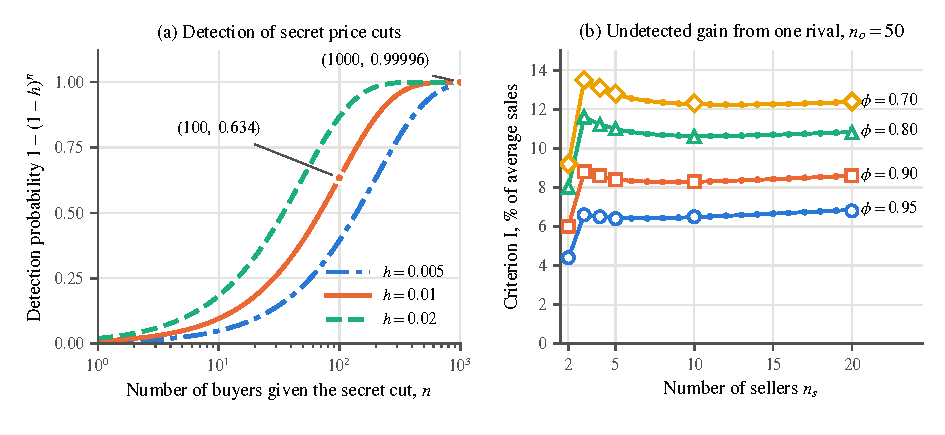
\includegraphics[width=\textwidth]{figures/ch02/stigler_detection.pdf}
\caption{Detection of secret price cutting. Panel (a) plots the probability that rivals hear of at least one secret cut
given to $n$ buyers, $1 - (1 - h)^n$, where $h$ is the probability that one cut is reported. The marked points are
Stigler's examples for $h = 0.01$. Panel (b) plots Stigler's Criterion I, \eqref{eq:02-stigler-crit1}, for $n_o = 50$
old buyers and four repeat probabilities $\phi$. Small dots are the formula at each integer $n_s$, and open markers
are the printed entries of \citet{Stigler1964}, Table 1. They coincide up to rounding.}
\label{fig:02-stigler-detect}
\end{figure}

\casehead{Criterion II: retaining one's own old customers}
A price cutter can also use secret cuts to keep more of its own old customers than usual. Without price cutting,
seller $i$ loses on average $(1 - \phi)\frac{n_o}{n_s}$ old customers, with variance $\sigma_1^2$. A single rival
has little basis for judging whether it receives a fair share of these. Stigler therefore assumes that the rivals
pool their information and suspect price cutting if seller $i$ loses fewer than
$(1 - \phi)\frac{n_o}{n_s} - 2\sigma_1$ customers, a 5 percent probability level. The cutter can then retain at most
$2\sigma_1$ extra old customers. As a share of its average sales, this is \emph{Criterion II},
\begin{equation}\label{eq:02-stigler-crit2}
G_{\mathrm{II}}(\phi, n_o, n_s) = \frac{2\sigma_1}{\frac{n_o}{n_s}} = 2\sqrt{\phi(1 - \phi)\,\frac{n_s}{n_o}} .
\end{equation}
It depends on the market only through the number of old customers per seller. Panel A of
\cref{tab:02-stigler-t234} reproduces part of Stigler's Table 2.

Comparing the two criteria shows that a price cutter is easier to detect through its gains from any one rival than
through an unusual rate of repeat sales. With $\phi = 0.95$ and 10 old customers per seller, Criterion II allows
13.8 percent. Table 1 gives the corresponding entries for one rival. They are 6.9 (2 sellers and 20 buyers), 8.9
(3 and 30), 7.4 (4 and 40), 6.4 (5 and 50) and 4.2 (10 and 100). Stigler adds two qualifications \citep[footnote 9]{Stigler1964}.
Multiplying the Table 1 entries by $n_s - 1$ gives the gain from all rivals together, which exceeds 13.8 percent
beyond two sellers. And Table 1 uses a looser probability level, so strict comparability would lower the Table 2
entries by one fifth. Stigler concludes that Criterion II will seldom be useful.

\casehead{Criterion III: new buyers}
New buyers form a flow rather than a stock, and Stigler takes the annual flow relative to old buyers as the unit.
Without price cutting, seller $i$ expects to sell to $m_3 = \frac{\lambda n_o}{n_s}$ new buyers, with binomial
variance $\sigma_3^2 = \left(1 - \frac{1}{n_s}\right)\frac{\lambda n_o}{n_s}$. Rivals cannot police this margin without
pooling information. With pooling, the seller is deemed a price cutter if it wins more than $m_3 + 2\sigma_3$ new
buyers, again a 5 percent level. Its total sales are $\frac{n_o(1 + \lambda)}{n_s}$ on average, so the largest
undetected gain as a share of sales is \emph{Criterion III},
\begin{equation}\label{eq:02-stigler-crit3}
G_{\mathrm{III}}(\lambda, n_o, n_s) = \frac{2\sigma_3}{\frac{n_o(1 + \lambda)}{n_s}}
= \frac{2}{1 + \lambda}\sqrt{\frac{(n_s - 1)\,\lambda}{n_o}} ,
\end{equation}
where the second equality uses $\sigma_3\frac{n_s}{n_o} = \sqrt{\frac{(n_s - 1)\lambda}{n_o}}$.

Panel B of \cref{tab:02-stigler-t234} reproduces part of Stigler's Table 3. The incentive to cut prices to new
buyers rises rapidly with the number of sellers, in proportion to $\sqrt{n_s - 1}$ for a given total of buyers. It
rises slowly when buyers per seller are held fixed. With $\lambda = \frac{1}{10}$ and 10 buyers per seller, it is
12.9 percent with 2 sellers and 17.7 percent with 20. It falls with the absolute number of buyers. Its dependence
on the rate of entry runs through the factor $\frac{\sqrt{\lambda}}{1 + \lambda}$, whose derivative has the sign of
$1 - \lambda$. The criterion therefore rises with $\lambda$ for $0 < \lambda < 1$, peaks at $\lambda = 1$ and falls
beyond it. With $n_o = 100$ and $n_s = 10$, it is 30 percent at $\lambda = 1$ and 24 percent at $\lambda = 4$. Rates
above one mean more new buyers per year than old buyers, and Stigler's Table 3 stays within $\lambda \le
\frac{1}{4}$. In that range, Stigler finds that when new buyers arrive at 10 percent per year or more, secret cuts
aimed at them yield larger undetected gains than poaching from any one rival. With $\phi = 0.90$, 100 old
buyers and 10 sellers, Criterion I allows 5.4 percent from each rival, while Criterion III with $\lambda =
\frac{1}{10}$ allows 17.2 percent in total. Markets in which new buyers arrive at such rates are therefore hard to
cartelize.

\begin{table}[htbp]
\centering
\caption{Stigler's Criteria II, III and IV (percent of average sales)}
\label{tab:02-stigler-t234}
\small
{\textit{Panel A. Criterion II: old customers a price cutter can retain (Table 2)}}\par\smallskip
\begin{tabular}{@{}lcccc@{}}
\toprule
& \multicolumn{4}{c}{Old customers per seller $\frac{n_o}{n_s}$} \\
\cmidrule(l){2-5}
Repeat probability $\phi$ & 10 & 20 & 50 & 100 \\
\midrule
0.95 & 13.8 & 9.7  & 6.2  & 4.4  \\
0.90 & 19.0 & 13.4 & 8.5  & 6.0  \\
0.80 & 25.3 & 17.9 & 11.3 & 8.0  \\
0.70 & 29.0 & 20.5 & 13.0 & 9.2  \\
0.50 & 31.6 & 22.4 & 14.1 & 10.0 \\
\bottomrule
\end{tabular}

\medskip
{\textit{Panel B. Criterion III: additional new customers obtainable (Table 3)}}\par\smallskip
\begin{tabular}{@{}cc*{6}{r}@{}}
\toprule
& & \multicolumn{6}{c}{Number of sellers $n_s$} \\
\cmidrule(l){3-8}
New-buyer rate $\lambda$ & Old buyers $n_o$ & 2 & 3 & 4 & 5 & 10 & 20 \\
\midrule
$\frac{1}{100}$ & 20  & 4.4 & 6.3 & 7.7 & 8.9 & 13.3 & 19.3 \\
                & 100 & 2.0 & 2.8 & 3.4 & 4.0 & 5.9  & 8.6  \\
                & 400 & 1.0 & 1.4 & 1.7 & 2.0 & 3.0  & 4.3  \\
\addlinespace
$\frac{1}{10}$  & 20  & 12.9 & 18.2 & 22.3 & 25.7 & 38.6 & 56.0 \\
                & 100 & 5.8  & 8.1  & 10.0 & 11.5 & 17.2 & 25.1 \\
                & 400 & 2.9  & 4.1  & 5.0  & 5.8  & 8.6  & 12.5 \\
\addlinespace
$\frac{1}{4}$   & 20  & 17.9 & 25.3 & 31.0 & 35.8 & 53.7 & 78.0 \\
                & 100 & 8.0  & 11.3 & 13.9 & 16.0 & 24.0 & 34.9 \\
                & 400 & 4.0  & 5.7  & 6.9  & 8.0  & 12.0 & 17.4 \\
\bottomrule
\end{tabular}

\medskip
{\textit{Panel C. Criterion IV: gain of a small firm against a large one, $\phi = 0.9$ (Table 4)}}\par\smallskip
\begin{tabular}{@{}cccccc@{}}
\toprule
& & \multicolumn{4}{c}{Size of large firm $K$} \\
\cmidrule(l){3-6}
Firms $n_s - K + 1$ & Buyers per small seller & 1 & 2 & 5 & 9 \\
\midrule
2  & 10 & 9.5 & 13.4 & 21.2 & 28.5 \\
2  & 50 & 4.2 & 6.0  & 9.5  & 12.7 \\
4  & 10 & 9.7 & 13.1 & 19.7 & 25.7 \\
10 & 10 & 5.4 & 7.2  & 10.7 & 14.0 \\
10 & 50 & 2.2 & 2.9  & 4.5  & 5.9  \\
\bottomrule
\end{tabular}

\medskip
\begin{minipage}{0.94\linewidth}
\footnotesize
Notes: Selected cells of \citet{Stigler1964}, Tables 2 to 4. Panel A uses \eqref{eq:02-stigler-crit2}, Panel B
uses \eqref{eq:02-stigler-crit3} and Panel C uses \eqref{eq:02-stigler-crit4}. We recomputed every printed cell of
the three tables. All agree to within 0.06 except one cell of Table 4 ($\phi = 0.9$, four firms, 50 buyers per
small seller, $K = 1$). It is printed as 4.0, while the formula gives 3.93 and the matching Table 1 cell is 3.9. In
Panel C, $n_s$ counts sellers in units of the small firm, so a firm of size $K$ counts as $K$ sellers.
\end{minipage}
\end{table}

\casehead{Pooling of information and unequal firm sizes}
With more than two sellers, firms can pool information and detect smaller deviations. The average number of old
customers that one cutter can take from $T$ rivals that pool information is at most
$\frac{T(1 - \phi)\,n_o}{n_s(n_s - T)}\bigl(1 + \frac{\tau}{\sqrt{T}}\bigr)$, with a correspondingly scaled variance.
For $T = 1$ this is $m_2$.
Both are smaller, relative to the customers lost by each pooling firm, than the corresponding expressions for one
seller. Pooling has limits. It becomes expensive as the pool grows, and it produces less reliable information,
because a member of the pool may itself be cutting prices.

Pooling by $K$ firms is equivalent to a single firm $K$ times as large as the others. Stigler's \emph{Criterion IV}
gives the gain of a small firm against such a large rival. It is measured as a percentage of the small firm's
average number of old customers, with $n_s$ counted in small-firm units:
\begin{equation}\label{eq:02-stigler-crit4}
G_{\mathrm{IV}} = \frac{1}{n_s - K}\left[\tau(1 - \phi)\sqrt{K}
+ \sqrt{\frac{n_sK(1 - \phi)(n_s - K - 1)\bigl(1 + \frac{\tau}{\sqrt{K}}\bigr)}{n_o}}\,\right].
\end{equation} For $K = 1$ it reduces to Criterion I. Compare Tables 1 and 4 for 100
customers, 10 firms and $\phi = 0.9$. A firm can take 5.4 percent of its sales from one rival, or about 50 percent
from all nine. If the nine rivals combine, Table 4 caps its gain at 28.5 percent.
In a second example with 20 firms and 200 customers, the gain from nine rivals falls from about 30 percent to 14.0
percent when they merge. Pooling information thus substantially reduces the scope for secret price cutting.
Stigler notes that Table 4 exaggerates the effect of size inequality. Only buyers above some size relative to the
seller are worth secret cuts, and a small firm can profitably cut prices to buyers too small to interest a large
seller.

\casehead{Repetition over time}
What may be chance in a single round cannot equally be chance if repeated. Over $T$ rounds, the mean loss to a
rival grows in proportion to $T$, while its standard deviation grows in proportion to $\sqrt{T}$. The threshold loss
over $T$ rounds is therefore $\frac{T(1 - \phi)}{n_s - 1}\cdot\frac{n_o}{n_s}\bigl(1 + \frac{\tau}{\sqrt{T}}\bigr)$.
The tolerated excess, relative to the mean, falls only as $\frac{1}{\sqrt{T}}$. Stigler concludes that this source of
information has minor efficacy unless buyers purchase, or sign contracts, frequently.

\subsubsection{Concentration and the Herfindahl index}

The model implies a measure of concentration suited to collusion. Suppose each new buyer picks firm $i$ with
probability equal to its output share $s_i$. Firm $i$'s number of new customers is then binomial with variance
$n_ns_i(1 - s_i)$. Summing over firms gives the total sampling noise against which price cutting must be detected,
\begin{equation}\label{eq:02-stigler-hhi}
\sum_{i} n_n s_i(1 - s_i) = n_n\Bigl(\sum_i s_i - \sum_i s_i^2\Bigr) = n_n(1 - \HHI) .
\end{equation}
The noise falls as the Herfindahl index rises. A similar argument applies to old customers
\citep[footnote 12]{Stigler1964}. Firm $j$ gains on average $(1 - \phi)n_o\frac{s_is_j}{1 - s_i}$ of the old customers
lost by firm $i$, with variance $(1 - \phi)n_o\frac{s_is_j}{1 - s_i}\bigl(1 - \frac{s_j}{1 - s_i}\bigr)$. Summing over
$i \ne j$ gives approximately $(1 - \phi)n_os_j(1 + \HHI - 2s_j)$. Summing over $j$ gives
$(1 - \phi)n_o(1 + \HHI - 2\HHI) = (1 - \phi)n_o(1 - \HHI)$. Stigler warns that the agreement of the two measures is
superficial, because the first assumes pooling of information and the second does not.

This gives a second foundation for the Herfindahl index, alongside the Cournot identity
$\bar L = \frac{\HHI}{\varepsilon}$ of \cref{prop:02-cowling-waterson}. The two arguments differ in kind. In Cournot,
a higher $\HHI$ raises margins under fixed noncooperative conduct. In Stigler's model, a higher $\HHI$ makes
collusion easier to police, so conduct itself changes. Both make the Herfindahl index more informative than a
four-firm ratio.

The analysis extends to nonprice competition with two modifications. There must be a definite joint
profit-maximizing policy to agree on, which is clearer for some variables than others. And nonprice moves differ in
detectability. Advertising, product quality and servicing leave visible traces, while reciprocal purchasing and
patent licensing do not. Collusion should suppress competition in the visible dimensions and leave it alive in the
hidden ones. The common belief that nonprice competition is more prevalent than price competition is therefore only
partly consistent with the theory.

The model's predictions can be collected. Collusion is easier to sustain when there are fewer sellers and when
buyers are numerous and small relative to sellers. A secret cut offered to many small buyers is likely to be
detected. Collusion is also easier when buyers are loyal ($\phi$ high) and new buyers arrive slowly ($\lambda$ low,
within $\lambda < 1$). It is easier still when sellers are unequal in size or pool information, when buyers report prices,
and when transactions are homogeneous enough for a simple price structure.

\subsubsection{Evidence}

Stigler's Section IV offers what he calls fragments of evidence. Two studies of the effect of the number of sellers
on price come first. He notes that, as far as he knows, no systematic analysis of this effect had been made
before.

\casehead{Newspapers and radio}
The first study concerns newspaper advertising rates in 53 cities in 1939. The rate per line per million
circulation, called the milline rate $R$, falls with circulation $z$. Stigler therefore first regresses
\begin{equation*}
\log R = 5.194 - \underset{(0.620)}{1.688}\,\log z + \underset{(0.063)}{0.139}\,(\log z)^2
\end{equation*}
He then tabulates the residuals by the number of evening papers in the city (Panel A of
\cref{tab:02-stigler-t56}). The mean residual is 0.0211 in one-paper cities and $-0.0213$ in two-paper cities.
Stigler reads this as rates about 5 percent above average in one-paper towns and 5 percent below in two-paper
towns. That reading matches base-10 logarithms, since $10^{0.0211} = 1.050$, while $e^{0.0211} = 1.021$.
Stigler adds that one-paper cities with an independent morning paper fall nearly midway between the two groups,
although their tabulated mean residual ($-0.0174$) lies close to the two-paper mean. Few cities had
more than two evening papers, so larger numbers of firms could not be studied. The subgroup means are internally
consistent: $\frac{10(-0.0174) + 13(0.0507)}{23} = 0.0211$.

The second study regresses the logarithm of AM radio spot rates on station characteristics for 345 stations in
Ohio, Indiana, Michigan and Illinois in 1961 (Panel B of \cref{tab:02-stigler-t56}). The elasticity of the rate with
respect to the number of stations in the county is $-0.074$, with a standard error of 0.046. The number of stations
ranges from 1 to 13 and is highly correlated with county population ($r^2 = 0.796$ in logarithms), which the
regression controls for. Both studies suggest that prices respond little to the number of rivals. Stigler finds this
consistent with his model, in which the number of buyers, the share of new buyers and the relative sizes of firms
matter as much as the number of sellers.

\begin{table}[htbp]
\centering
\caption{Number of sellers and prices in Stigler (1964)}
\label{tab:02-stigler-t56}
\small
{\textit{Panel A. Residuals from the regression of newspaper advertising rates on circulation, 1939 (Table 5)}}\par\smallskip
\begin{tabular}{@{}lccc@{}}
\toprule
Evening papers in city & Cities & Mean residual & Standard deviation of mean \\
\midrule
One                          & 23 & $0.0211$  & 0.0210 \\
\quad With morning paper     & 10 & $-0.0174$ & 0.0324 \\
\quad Without morning paper  & 13 & $0.0507$  & 0.0233 \\
Two                          & 30 & $-0.0213$ & 0.0135 \\
\bottomrule
\end{tabular}

\medskip
{\textit{Panel B. Regression of log AM spot commercial rates, 1961, $n = 345$ (Table 6)}}\par\smallskip
\begin{tabular}{@{}lcc@{}}
\toprule
Regressor & Coefficient & Standard error \\
\midrule
Log population of county, 1960              & $0.238$  & 0.026 \\
Log kilowatt power of station               & $0.206$  & 0.015 \\
Broadcast period: sunrise to sunset         & $-0.114$ & 0.025 \\
Broadcast period: longer, under 18 hours    & $-0.086$ & 0.027 \\
Broadcast period: 18 to 21 hours            & $-0.053$ & 0.028 \\
Log number of stations in county            & $-0.074$ & 0.046 \\
\midrule
$R^2$ & \multicolumn{2}{c}{0.743} \\
\bottomrule
\end{tabular}

\medskip
\begin{minipage}{0.94\linewidth}
\footnotesize
Notes: From \citet{Stigler1964}, Tables 5 and 6. Panel A: residuals, in logarithms, from
$\log R = 5.194 - 1.688\log z + 0.139(\log z)^2$, where $R$ is the milline rate and $z$ is circulation. The standard
errors of the slope coefficients are 0.620 and 0.063. Stigler's data come from the American Association of
Advertising Agencies. Panel B: the dependent variable is the logarithm of the average rate for 26 spots on May 1, 1961. The
broadcast-period variables are dummies. Table 6 does not state the omitted category. Stigler's data come from
the Standard Rate and Data Service.
\end{minipage}
\end{table}

\casehead{Profitability and concentration}
The direct test of the theory relates profitability to concentration across industries. Stigler restricts the
sample to 17 industries in which the sampled firms account for at least 35 percent of industry sales and earn at
least half of their revenue in the industry. Large steel and chemical firms, for example, operate in many markets
and are excluded. \Cref{tab:02-stigler-t7} reproduces his Table 7. Concentration in 1954 is measured by the four-firm
share and by the Herfindahl index. Profitability over 1953--57 is measured by the rate of return on all assets, the
rate of return on net worth, and the ratio of market to book value of common stock.

\begin{table}[htbp]
\centering
\begin{threeparttable}
\caption{Profitability and concentration in 17 industries (Stigler 1964)}
\label{tab:02-stigler-t7}
\small
\begin{tabular}{@{}lccccc@{}}
\toprule
& \multicolumn{2}{c}{Concentration, 1954} & \multicolumn{2}{c}{Average return, 1953--57} & Market to book \\
\cmidrule(lr){2-3}\cmidrule(lr){4-5}
Industry (firms) & Top-4 share & $\HHI$ & All assets & Net worth & value, 1953--57 \\
\midrule
\multicolumn{6}{@{}l}{\textit{Panel A. Industry data (Table 7)}} \\
Sulfur mining (4)                  & 98 & 0.407 & 19.03 & 23.85 & 3.02 \\
Automobiles (3)                    & 98 & 0.369 & 11.71 & 20.26 & 2.30 \\
Flat glass (3)                     & 90 & 0.296 & 11.79 & 16.17 & 2.22 \\
Gypsum products (2)                & 90 & 0.280 & 12.16 & 20.26 & 1.83 \\
Primary aluminum (4)               & 98 & 0.277 & 6.87  & 13.46 & 2.48 \\
Metal cans (4)                     & 80 & 0.260 & 7.27  & 13.90 & 1.60 \\
Chewing gum (2)                    & 86 & 0.254 & 13.50 & 17.06 & 2.46 \\
Hard-surface floor coverings (3)   & 87 & 0.233 & 6.56  & 7.59  & 0.98 \\
Cigarettes (5)                     & 83 & 0.213 & 7.23  & 11.18 & 1.29 \\
Industrial gases (3)               & 84 & 0.202 & 8.25  & 11.53 & 1.33 \\
Corn wet milling (3)               & 75 & 0.201 & 9.17  & 11.55 & 1.48 \\
Typewriters (3)                    & 83 & 0.198 & 3.55  & 5.39  & 0.84 \\
Domestic laundry equipment (2)     & 68 & 0.174 & 9.97  & 17.76 & 1.66 \\
Rubber tires (9)                   & 79 & 0.171 & 7.86  & 14.02 & 1.70 \\
Rayon fiber (4)                    & 76 & 0.169 & 5.64  & 6.62  & 0.84 \\
Carbon black (2)                   & 73 & 0.152 & 8.29  & 9.97  & 1.40 \\
Distilled liquors (6)              & 64 & 0.118 & 6.94  & 7.55  & 0.77 \\
\midrule
\multicolumn{6}{@{}l}{\textit{Panel B. Rank correlations with profitability (Table 8)}} \\
Top-4 share      & & & 0.322 & 0.507 & 0.642 \\
Herfindahl index & & & 0.524 & 0.692 & 0.730 \\
\bottomrule
\end{tabular}
\begin{tablenotes}\footnotesize
\item Notes: From \citet{Stigler1964}, Tables 7 and 8. The number of sampled firms is in parentheses. Returns are in
percent. In Panel B, each entry is the rank correlation between the concentration measure in the row and the
profitability measure in the column. Stigler reports a rank correlation of 0.903 between the two concentration
measures (his footnote 14). Our Spearman correlations computed from Panel A are 0.320, 0.499 and 0.652 for the
top-4 share. For $\HHI$ they are 0.525, 0.692 and 0.737, and between the two measures 0.903. The small differences
presumably reflect the treatment of ties.
\end{tablenotes}
\end{threeparttable}
\end{table}

All six rank correlations are positive. The Herfindahl index correlates more strongly with each profitability
measure than the four-firm share does, as the variance argument of \eqref{eq:02-stigler-hhi} suggests. Stigler
reads the data as showing no relation between profitability and concentration when $\HHI$ is below 0.250 or the
four-firm share is below about 80 percent. Our computations from Table 7 agree. Among the ten industries with
$\HHI < 0.250$, the Spearman correlations of $\HHI$ with the three profitability measures are $-0.03$, 0.18 and
0.11. The seven industries above the threshold earn on average 11.8 percent on assets, against 7.3 percent below
it. Stigler is careful about what this shows. The data, like those on advertising rates, ``confirm our theory only
in the sense that they support theories which assert that competition increases with number of firms.''

\casehead{Price cutting in steel}
The last piece of evidence uses prices paid by buyers of steel products in the second quarter of 1939, measured
relative to quoted prices. \Cref{tab:02-stigler-t9} reproduces Stigler's Table 9. The entry of 8.3 for hot-rolled
sheets, for example, is an average reduction of 8.3 percent from quoted prices, with a standard deviation of 7.3
percent of quoted prices. The average discount is almost perfectly correlated with the dispersion of transaction
prices. Our correlation across the eight products is 0.91. Stigler interprets this as expected: the less perfect the
market knowledge, the more extensive the price cutting.

\begin{table}[htbp]
\centering
\begin{threeparttable}
\caption{Prices of steel products and industry structure (Stigler 1964)}
\label{tab:02-stigler-t9}
\small
\begin{tabular}{@{}lcccc@{}}
\toprule
& \multicolumn{2}{c}{Prices, 2nd quarter 1939 (percent)} & & \\
\cmidrule(lr){2-3}
Product class & Average discount & Standard deviation & Herfindahl index & Output 1939 \\
& from list price & & & relative to 1937 \\
\midrule
Hot-rolled sheets   & 8.3 & 7.3 & 0.0902 & 1.14 \\
Merchant bars       & 1.2 & 4.5 & 0.1517 & 0.84 \\
Hot-rolled strip    & 8.5 & 8.3 & 0.1069 & 0.56 \\
Plates              & 2.6 & 4.8 & 0.1740 & 0.85 \\
Structural shapes   & 3.2 & 4.3 & 0.3280 & 0.92 \\
Cold-rolled strip   & 8.8 & 9.8 & 0.0549 & 0.88 \\
Cold-rolled sheets  & 5.8 & 5.0 & 0.0963 & 1.14 \\
Cold-finished bars  & 0.9 & 3.4 & 0.0964 & 0.83 \\
\bottomrule
\end{tabular}
\begin{tablenotes}\footnotesize
\item Notes: From \citet{Stigler1964}, Table 9, in his row order. The Herfindahl index uses 1938 capacity.
Transaction prices come from a Bureau of Labor Statistics survey reported in \textit{Iron Age} (1946). Capacity
data come from the \textit{Directory of Iron and Steel Works of the United States and Canada}, and output data
from the American Iron and Steel Institute. In our computations across the eight rows, the correlation of the
discount with its standard deviation is 0.91. The correlation of the discount with $\HHI$ is $-0.46$ (Spearman
$-0.55$), and the least-squares line is $\text{discount} = 7.40 - 18.09\,\HHI$.
\end{tablenotes}
\end{threeparttable}
\end{table}

The data show larger discounts in the less concentrated product classes. Cold-rolled strip has the lowest index,
0.0549, and the largest discount, 8.8 percent. Structural shapes have the highest index, 0.3280, and a discount of
3.2 percent. This is the ordering the theory predicts, since secret cuts are harder to police when sellers are
numerous and small. Stigler's summary sentence states the relation with the opposite sign. His remarks on
individual products fit the data. He notes that structural shapes and hot-rolled strip sold somewhat below the
average relationship, while cold-finished bars sold above it. In our fitted line, the first two have discounts 1.7
and 3.0 points above the line and cold-finished bars 4.8 points below. He adds that the deviations are not
explained by demand, measured by 1939 output relative to 1937. Our residuals are indeed uncorrelated with that
measure. The survey also excluded some very large buyers in the automobile and container industries. Since very
large buyers obtained the largest concessions, Stigler infers that the table understates price cutting.

Stigler judged these fragments ``fairly favorable to the theory,'' while granting that they do not constitute strong
support. He expected more powerful tests from the electrical equipment conspiracy cases then in the courts. The
theory predicts that prices on public bids will be higher and less dispersed than in privately negotiated sales.
It also predicts that price cutting increases as the number of buyers diminishes \citep[footnote 16]{Stigler1964}. He saw the
large number of testable hypotheses as the main merit of the theory.

\subsubsection{Assessment}

Stigler's paper made collusion an information problem. It gave the first systematic account of why cartels hold in
some markets and fail in others, and it tied cartel stability to observable features of markets. These include the
number and size distribution of sellers, the size and loyalty of buyers and the rate of arrival of new buyers.
They also include the transparency of transaction prices and the complexity of the price structure. Several of these ideas now organize
antitrust thinking about coordinated effects, from the role of large buyers to the danger of price transparency
(\cref{ch:collusion-evidence}).

The model has clear limits. It contains no equilibrium. Punishment after detection is asserted, as the matching of
detected cuts, and never derived. The price cutter does not choose how much to cut by weighing gains against the
risk of detection. The detection rules use fixed probability thresholds, such as one standard deviation, without a
decision-theoretic basis. The collusive price level is not determined, and the criteria measure the incentive to cut
by undetected sales alone, ignoring the margin on those sales. The evidence is cross-sectional and inherits the
endogeneity of market structure discussed in \cref{ch:intro}.

\citet{GreenPorter1984} read Stigler differently from the cross-industry tradition he inspired (pp.~87--88). In their
reading, Stigler justified cross-industry regressions by relating concentration informally to a cartel's ability to
deter cheating, and by assuming that profitability reflects cartel success. They recast his cartel as the solution
to a design problem: an institution that achieves an efficient outcome subject to the constraint that members act
noncooperatively. That shift leads directly to the repeated-game models of the next subsection.

\subsection{Repeated interaction: a preview}\label{sec:02-repeated}

Repeated interaction gives Stigler's enforcement a formal foundation. A deviation today can be punished tomorrow,
so collusive prices can be an equilibrium even though each firm gains by deviating in the short run. As in
\cref{sec:02-multiproduct} and \cref{ch:collusion-theory}, $\delta \in (0, 1)$ denotes the discount factor. The
stage game is played in periods $t = 0, 1, 2, \dots$, and each firm maximizes $\sum_{t \ge 0}\delta^t\pi_{it}$. We
use \emph{grim-trigger strategies}: firms play the collusive action as long as no one has deviated, and revert
forever to the static Nash equilibrium after any deviation \citep{Friedman1971}. Static Nash play forever is itself
a subgame-perfect equilibrium, so the threat is credible. The one-shot deviation principle, the folk theorem and
optimal punishments are developed in \cref{ch:collusion-theory}.

The horizon must be infinite \citep[sec.~11.3.2]{Tirole1988}. A repeated game has almost perfect information
(\cref{sec:02-spe}), so it can be solved by backward induction when it ends at a known date. If the stage game has a
unique Nash equilibrium, the stage equilibrium is then played in every period, and collusion unravels from the end
(\cref{prop:12-finite}). The Bertrand game has several equilibrium profiles, but all of them give zero profit, so the
same argument applies. With an infinite horizon there is no last period from which to start. Repeating the stage
equilibrium forever remains a subgame-perfect equilibrium, because no current action changes future play. Other
equilibria now exist, and they are sustained by the threat of reverting to the stage equilibrium after a deviation.
\Cref{prop:02-bertrand-collusion,prop:02-cournot-collusion} state when this threat suffices. We give the intuition
here and prove both results in \cref{sec:12-perfect}.

\begin{proposition}[Collusion in the Bertrand supergame]\label{prop:02-bertrand-collusion}
Let $N$ identical firms with constant marginal cost $c$ play the homogeneous Bertrand game of \cref{sec:02-bertrand}
in every period, with observed prices. Grim-trigger strategies with collusive price $p^m$ and Bertrand reversion form
a subgame-perfect equilibrium if and only if
\begin{equation}\label{eq:02-bertrand-ic}
\delta \ge 1 - \frac{1}{N} .
\end{equation}
\end{proposition}

\Cref{prop:12-bertrand} gives the proof. On the collusive path, conforming yields $\frac{\pi^m}{N}$ in every period,
worth $\frac{\pi^m}{N(1 - \delta)}$. The best deviation undercuts $p^m$ slightly, earns almost $\pi^m$ once, and
earns zero after the reversion to Bertrand pricing. Collusion is sustainable when $\frac{\pi^m}{N(1 - \delta)} \ge
\pi^m$, which is \eqref{eq:02-bertrand-ic}.

The threshold rises with $N$. Each firm's collusive share $\frac{\pi^m}{N}$ shrinks while the one-period gain from
deviation stays at about $\pi^m$. This is the formal version of Stigler's observation that collusion is impossible
for many firms. \citet[sec.~6.3.2.1]{Tirole1988} uses it to give Bain's link between concentration and tacit
collusion a precise sense.

\begin{example}[Detection lags]\label{ex:02-detection-lag}
Stigler's insight is that deviations are detected with delay. Suppose rivals learn of a secret price cut only with
probability $\mu \in (0, 1]$ in each period, for instance because random switching of buyers masks the lost sales.
Until detection, the cutter serves the market at a price just below $p^m$. Its deviation payoff becomes
\begin{equation*}
\pi^m\sum_{t \ge 0}\bigl[\delta(1 - \mu)\bigr]^t = \frac{\pi^m}{1 - \delta(1 - \mu)} .
\end{equation*}
Conforming is optimal if and only if
\begin{equation*}
\frac{\pi^m}{N(1 - \delta)} \ge \frac{\pi^m}{1 - \delta + \delta\mu}
\iff \delta\mu \ge (N - 1)(1 - \delta)
\iff \delta \ge \frac{N - 1}{N - 1 + \mu} .
\end{equation*}
With $\mu = 1$ this is \eqref{eq:02-bertrand-ic}. As $\mu \to 0$ the threshold tends to 1, and collusion becomes
impossible. If a cut reaches 100 buyers who each report it with probability $h = 0.01$, then
$\mu = 1 - (0.99)^{100} = 0.634$ from \eqref{eq:02-stigler-detect}. The threshold rises from 0.50 to 0.61 for
two firms and from 0.80 to 0.86 for five.
\end{example}

\begin{proposition}[Collusion in the linear Cournot supergame]\label{prop:02-cournot-collusion}
Let $N$ identical firms with constant marginal cost $c$ play the Cournot game with $P(Q) = a - bQ$ in every period.
Grim-trigger strategies with collusive output $\frac{Q^m}{N}$ each and reversion to the Cournot equilibrium form a
subgame-perfect equilibrium if and only if
\begin{equation}\label{eq:02-cournot-delta}
\delta \ge \delta^*(N) = \frac{(N + 1)^2}{N^2 + 6N + 1} .
\end{equation}
\end{proposition}

\Cref{prop:12-cournot} gives the proof. Let $\pi_c$, $\pi_d$ and $\pi_n$ be the per-period collusive, best
one-shot deviation and Cournot profits. A firm conforms if collusion forever is worth at least one period of
deviation profit followed by Cournot profit forever:
\begin{equation*}
\frac{\pi_c}{1 - \delta} \ge \pi_d + \frac{\delta\,\pi_n}{1 - \delta}
\iff \delta \ge \frac{\pi_d - \pi_c}{\pi_d - \pi_n} .
\end{equation*}
With linear demand the three profits are proportional to $\frac{(a - c)^2}{b}$, so the ratio depends only on $N$. It
simplifies to \eqref{eq:02-cournot-delta}.

The threshold is $\delta^*(2) = \frac{9}{17} = 0.529$, and it rises to 0.571, 0.643 and 0.752 for $N = 3, 5$ and
10. Its derivative is $\frac{4(N - 1)(N + 1)}{(N^2 + 6N + 1)^2} > 0$, and $\delta^*(N) \to 1$ as $N \to \infty$. The
comparison with Bertrand is instructive. For $N = 2$ the Cournot threshold is higher than the Bertrand value of
0.5. For $N \ge 3$ it is lower: 0.571 against 0.667 at $N = 3$, and 0.752 against 0.900 at $N = 10$. Two forces
work in opposite directions. Cournot reversion is a milder punishment than Bertrand reversion. But a Cournot
deviator cannot capture the whole market, because rivals' outputs stay fixed. With three or more firms the second
force dominates.

\casehead{Conduct as a reduced form of dynamic play}
In these models the static conduct parameter of \cref{sec:02-conduct} summarizes the outcome of dynamic play. It is
close to 1 in collusive phases and close to its Cournot or Bertrand value in punishment phases. \citet{Bresnahan1989}
draws the empirical implication directly from Stigler (pp.~1023--1025). If self-interest alone holds a collusive
arrangement together, uncertainty about rivals' behavior will sometimes trigger price wars even without actual
cheating. Data on a collusive industry should then show periods of cooperation and periods of competition.
``Empirically, of course, this will show up as time-varying $\theta$.'' Two models formalize the idea with
different predictions about when the price wars occur.

\casehead{Green and Porter: price wars after bad news}
\citet{GreenPorter1984} study cartel self-enforcement under demand uncertainty. In their model firms choose outputs,
and the market price depends on total output and an unobserved demand shock. Firms observe the price, but neither
rivals' outputs nor the shock. A low price may therefore signal either cheating or bad demand. The cartel uses a
trigger price. Firms produce collusive outputs while the price stays above the trigger and revert to Cournot output
for a fixed number of periods after it falls below. In equilibrium no firm cheats, yet low demand realizations set
off price wars. The wars are necessary, because without them cheating could not be deterred. Green and Porter
emphasize that earlier formulations make incentives so perfect that the deterrent mechanism is never observed. With
imperfect information, recurrent price wars are part of successful collusion. They need not indicate a sequence of
failed attempts to form a cartel (pp.~87--88).

A simple price-setting version conveys the logic. Two firms face demand $Q(p)$ with probability $1 - \zeta$ and
zero demand with probability $\zeta$, independently each period. A firm with zero sales cannot tell low demand from
a rival's secret cut. The strategy is to price at $p^m$ until a period of zero sales and then price at $c$
forever. The value of collusion is $V = \frac{(1 - \zeta)\frac{\pi^m}{2}}{1 - \delta(1 - \zeta)}$. A deviator earns
$(1 - \zeta)\pi^m$ once and nothing afterwards. Conforming is optimal if and only if
\begin{equation*}
\frac{(1 - \zeta)\frac{\pi^m}{2}}{1 - \delta(1 - \zeta)} \ge (1 - \zeta)\,\pi^m
\iff \delta(1 - \zeta) \ge \frac{1}{2} .
\end{equation*}
More noise ($\zeta$ higher) makes collusion harder, and price wars start after unexpectedly low demand.
\Cref{ch:collusion-theory} treats finite punishments and the optimal trigger, including the refinements of
\citet{AbreuPearceStacchetti1986}.

\casehead{Rotemberg and Saloner: price wars during booms}
\citet{RotembergSaloner1986} study implicitly colluding oligopolists facing fluctuating demand that they observe.
Their key finding is that the temptation to deviate from the collusive outcome is often greater when demand is high.
To moderate the temptation, the oligopoly lowers its prices in booms. Suppose demand states are independent over
time, and let $\pi_s(p)$ be industry profit at price $p$ in state $s$. With collusive prices $p_s$ and Bertrand
reversion, the incentive constraint in state $s$ is
\begin{equation*}
\left(1 - \frac{1}{N}\right)\pi_s(p_s) \le \frac{\delta}{1 - \delta}\cdot\frac{1}{N}\,\E\bigl[\pi_{s'}(p_{s'})\bigr] .
\end{equation*}
The left side is the gain from deviating in the current state, and it rises with current demand. The right side is
the expected future loss, which does not depend on the current state. In high-demand states the constraint binds
first, and the cartel must cap profits below the monopoly level by cutting price. The abstract of the 1984 working-paper
version cites supporting evidence from the railroads in the 1880s and the automobile industry in the 1950s. It
also cites the cyclical behavior of cement prices and price-cost margins.

\casehead{Implications for measurement}
Both models imply that conduct varies over time, but they disagree about the pattern. In Green and Porter, conduct
switches to the competitive value after unanticipated low demand and returns after a fixed lag. In Rotemberg and
Saloner, conduct varies within the collusive regime with the level of demand. \citet{Porter1983} estimated a supply
relation with two regimes for a nineteenth-century railroad cartel (\cref{ch:collusion-evidence}). Bresnahan notes
that the existence of regimes is easier to establish than their causes. Asking whether there are price wars uses all
periods of data, while asking what starts and stops them has as many observations as there are wars. Time variation
in conduct also complicates the interpretation of a constant estimated $\theta$, which is the critique of
\citet{Corts1999} developed in \cref{ch:conduct}.

\section{From homogeneous to differentiated products}\label{sec:02-bridge}

The theory so far assumed a homogeneous good. Few markets fit that description. Products differ in physical
characteristics, location, brand and service, even in markets that look homogeneous, such as pharmaceuticals with
chemically identical generics or retail gasoline. Electricity and refined sugar, the settings of two case studies in
\cref{ch:conduct}, come close to homogeneity. Most empirical questions in industrial organization need a model of
demand for differentiated products. Measuring market power, evaluating mergers, assessing taxes and tariffs,
analyzing product introductions and valuing new goods all depend on substitution patterns. With differentiated
products there is also no natural boundary for the market, so an estimated demand system can stand in for
market definition. This section shows how the pricing logic of this chapter carries over and points to where it is
developed.

A single-product firm $j$ that sets its price, taking rivals' prices as given, is a monopolist on its residual
demand $q_j(p)$, as in \cref{sec:02-residual}. The first-order condition
$q_j + (p_j - mc_j)\frac{\partial q_j}{\partial p_j} = 0$ gives the dollar markup and Lerner rules
\eqref{eq:02-dollar-markup} and \eqref{eq:02-lerner}, with the own-price derivative of residual demand in place
of the market derivative:
\begin{equation}\label{eq:02-single-product-markup}
p_j - mc_j = -\frac{q_j}{\frac{\partial q_j}{\partial p_j}} ,
\qquad
\frac{p_j - mc_j}{p_j} = \frac{1}{|\varepsilon_{jj}|} .
\end{equation}
For example, with logit demand and price coefficient $\alpha$, $\frac{\partial s_j}{\partial p_j} = -\alpha s_j(1 - s_j)$,
so the markup is $\frac{1}{\alpha(1 - s_j)}$. Pass-through follows the formulas of \cref{sec:02-passthrough}, and for
the logit it equals $1 - s_j$ when rivals' prices are held fixed (\cref{ex:02-pt-examples}).

A firm that owns several products adds a new term. Let firm $f$ own the set $\mathcal{J}_f$ and maximize
$\sum_{k \in \mathcal{J}_f}(p_k - mc_k)\,q_k(p)$ over its own prices. The first-order condition for $p_j$,
$j \in \mathcal{J}_f$, is
\begin{equation*}
q_j + (p_j - mc_j)\frac{\partial q_j}{\partial p_j} + \sum_{k \in \mathcal{J}_f\setminus\{j\}}(p_k - mc_k)\frac{\partial q_k}{\partial p_j} = 0 .
\end{equation*}
Divide by $\frac{\partial q_j}{\partial p_j} < 0$, solve for $p_j$, and define the \emph{diversion ratio}
$D_{jk} = -\frac{\partial q_k}{\partial p_j}\bigl(\frac{\partial q_j}{\partial p_j}\bigr)^{-1}$, the fraction of the sales lost by
product $j$ that product $k$ recaptures when $p_j$ rises. Then
\begin{equation}\label{eq:02-diversion-foc}
p_j = mc_j - \frac{q_j}{\frac{\partial q_j}{\partial p_j}} + \sum_{k \in \mathcal{J}_f\setminus\{j\}}(p_k - mc_k)\,D_{jk} .
\end{equation}
Price equals marginal cost, plus the single-product markup, plus the margins the firm earns on sales recaptured by
its other products. The last term is an opportunity cost of selling product $j$, since each sale partly
cannibalizes the firm's other products. Joint ownership of substitutes therefore raises prices. A merger adds the
acquired products to $\mathcal{J}_f$ and the corresponding terms to \eqref{eq:02-diversion-foc}. This is the logic
of upward pricing pressure in \cref{ch:mergers}. The homogeneous-goods analogue is the gap between Cournot conduct,
in which each firm ignores its effect on rivals, and collusion, in which it internalizes all of it
(\cref{prop:02-cheat}).

When one firm owns every product, this first-order condition is the condition \eqref{eq:02-multi-foc-margin} of the
multiproduct monopolist in \cref{sec:02-multiproduct}. The diversion-ratio form is the same condition divided by
the own-price derivative. To see the link with the Lerner form, substitute $\frac{\partial q_k}{\partial p_j} =
\varepsilon_{kj}\frac{q_k}{p_j}$ and $\frac{\partial q_j}{\partial p_j} = -\lvert\varepsilon_{jj}\rvert\frac{q_j}{p_j}$
into the definition of the diversion ratio:
\[
  D_{jk} = \frac{\varepsilon_{kj}\,q_k}{\lvert\varepsilon_{jj}\rvert\,q_j} .
\]
The single-product markup is $-q_j\bigl(\frac{\partial q_j}{\partial p_j}\bigr)^{-1} =
\frac{p_j}{\lvert\varepsilon_{jj}\rvert}$.
Dividing \eqref{eq:02-diversion-foc} by $p_j$ and writing $R_j = p_jq_j$ then gives
\[
  \frac{p_j - mc_j}{p_j} = \frac{1}{\lvert\varepsilon_{jj}\rvert}
  + \sum_{k \in \mathcal{J}_f\setminus\{j\}}\frac{(p_k - mc_k)\,q_k\,\varepsilon_{kj}}{R_j\,\lvert\varepsilon_{jj}\rvert} ,
\]
which is \eqref{eq:02-multi-lerner} with the sum restricted to the firm's own products. Positive diversion
corresponds to substitutes in that formula, and it raises the Lerner index above the inverse own elasticity.

Stacking \eqref{eq:02-diversion-foc} over products gives the matrix form $p = mc - (\Omega \odot \Delta^\top)^{-1}q$,
with ownership matrix $\Omega$ ($\Omega_{jk} = 1$ if $j$ and $k$ have the same owner) and demand Jacobian $\Delta$,
whose $(j,k)$ element is $\frac{\partial q_j}{\partial p_k}$. \Cref{ch:diffprod} develops this system, the existence
and uniqueness of equilibrium, the recovery of marginal costs from estimated demand, and the demand models that
supply the derivatives. Theory in this area mostly studies prices and products given a demand system. Empirical work
does the reverse: it models demand richly and supply simply, usually as static Bertrand-Nash pricing. Richer demand
models add assumptions and computation, so they should be judged by what they add for the question at hand and the
data available.
